\documentclass[letterpaper]{article}
\usepackage{natbib,alifeconf}
\usepackage{hyperref}
\usepackage{tablefootnote}

\title{The MODES Toolbox: Measurements of Open-ended Dynamics in Evolving Systems}
\author{Emily L. Dolson$^{1,2,3}$, Anya E. Vostinar$^{4}$, Michael J. Wiser$^{1,3}$,\and Charles Ofria$^{1,2,3}$ \\
\mbox{}\\
$^1$BEACON Center for the Study of Evolution in Action  \\
$^2$Department of Computer Science and Engineering, Michigan State University, MI, 48823 \\
$^3$Program in Ecology, Evolutionary Biology, and Behavior, Michigan State University, MI, 48823 \\
$^4$Grinnell College, Grinnell, IA, 50112 \\
dolsonem@msu.edu}


\begin{document}
\maketitle

\section{Abstract}

Building more open-ended evolutionary systems can simultaneously advance our understanding of biology, artificial life, and evolutionary computation. In order to do so, however, we need a way to determine when we are moving closer to this goal. We propose a set of metrics that allow us to measure commonly-agreed-upon hallmarks of open-ended evolution in a system: change potential, novelty potential, complexity potential, and ecological potential. Our goal is to make these metrics easy to incorporate into a system, and comparable across systems so that we can make coherent progress as a field. To this end, we provide a C++ implementation of these metrics that should be easy to connect to existing artificial life systems. As the field reaches consensus about additional hallmarks of open-ended evolution, metrics corresponding to these additions can be added to this toolbox. For example, we hope to soon add a measurement of the potential for major transitions in individuality to occur. To confirm that our metrics accurately measure the hallmarks we are interested in, we test them on two very different experimental systems: NK Landscapes and the Avida Digital Evolution Platform. We find that our observed results are consistent with our prior knowledge about these systems, suggesting that our proposed metrics are effective and should generalize to other systems.
% @ELD: I'm having trouble working this last point in:
% Two key components to any OEE metric: What do we call ``components'' of the system, and how do we ensure that we only focus on meaningful components that have been selected by evolution?

\section{Introduction}

A central goal of the field of artificial life is to build evolving systems that capture the full range of dynamics from nature. Such systems should be capable of producing evolutionary outcomes such as sophisticated navigation behaviors, novel cooperative strategies, complex ecosystems, or major evolutionary transitions, to name but a few. Researchers seek such ``open-ended'' systems for a number of reasons:
1) For biologists, access to systems exhibiting complex and nuanced evolutionary processes allows rapid experimentation and facilitates developing a deep intuition for underlying mechanisms \citep{tenaillon_tempo_2016}.
2) For evolutionary computation researchers, insights from open-ended evolutionary systems will allow researchers to break complexity barriers, expanding the classes of engineering problems that evolutionary algorithms can solve \citep{Hara:1999vo, Potter:2000dw} and producing more general forms of evolved intelligence.
3) For artificial life researchers, the presence of dynamics that are seen in biology but not in artificial life indicates that we are not yet sure how to build evolving systems as innovative as those found in nature, be it due to limited memory, limited time, or simply an insufficient understanding of the necessary components.
Identifying these missing factors should allow us to better understand life as it is and to better explore life as it could be.

While various artificial life systems have reproduced individual dynamics -- such as the evolution of complex traits \citep{Lenski:2003vy}, cooperative behaviors \citep{Goldsby:2012tz}, and coexistence of diverse ecotypes \citep{cooper_evolution_2003} -- these accomplishments have been in highly controlled circumstances. The overarching goal of open-ended evolution research is to create a system where all of these dynamics can emerge more organically, as in the biosphere. 
Additionally, replicating this process would provide incredible insights into our own origins, including the evolution of human intelligence.  Indeed harnessing a more open-ended set of evolutionary dynamics could help us spur breakthroughs in the evolution of general artificial intelligence.

\begin{figure}
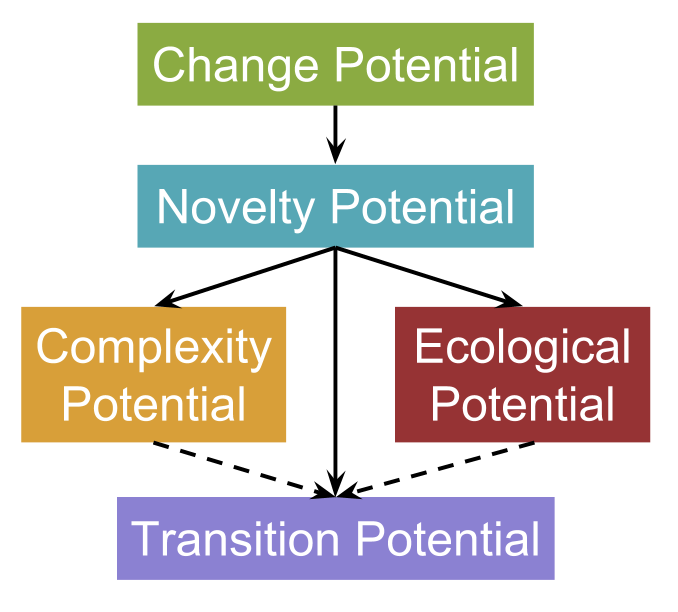
\includegraphics[width=3.5in]{figs/Complexity_Barriers.png}
\caption{\textbf{Relationships between the metrics.} Originally published in \citep{blogpost}. Solid lines with arrows indicate metrics which are prerequisites for other metrics.}
\label{hierarchy}
\end{figure}

Open-ended evolution is a many-faceted concept. A number of patterns are considered to be hallmarks of open-ended evolution \citep{taylor_open-ended_2016}, most notably the continual production of novelty \citep{lehman_abandoning_2011, banzhaf_defining_2016}, unconstrained increases in diversity \citep{bedau1994bifurcation}, ongoing increases in complexity \citep{Lenski:2003vy, Korb:2011kg}, and shifts in individuality such as those often associated with major transitions in evolution \citep{smith1997major}. There is a growing consensus in the field that all of these dynamics are important pieces of the open-ended evolution puzzle \citep{taylor_open-ended_2016}. In addition, we have previously suggested that there is a fifth necessary and even simpler dynamic: continuous change in the population \citep{blogpost}.


These five properties of a system fit into a hierarchy, as shown in Figure \ref{hierarchy}. For novelty to exist, there must be some degree of change in the information within a population. While this is trivially true, many evolutionary algorithms suffer from premature convergence, which is essentially the absence of non-trivial change, so it remains an important prerequisite to define and explicitly address. Similarly, complexity and diversity can only increase indefinitely if novel members of the population continue to be generated. Finally, transitions in individuality typically involve multiple organisms coming together into a single individual, building from complex and diverse progenitors.  All of these dynamics capture different subsets of interesting behavior that an evolving system might exhibit and we propose they are all necessary (but perhaps not sufficient) in a fully open-ended system.

To draw conclusions about what factors of a system promote or inhibit these dynamics, we need methods for measuring the extent to which each dynamic is present. Importantly, these methods must be applicable across a wide variety of systems. Some progress has been made toward this end with evolutionary activity statistics \citep{bedau_classification_1998, channon_passing_2001}, an approach to isolating and quantifying the adaptive component of an evolving system, separating out the non-adaptive dynamics. Evolutionary activity statistics require that the user decide on two things ahead of time: a definition for ``components'' (meaningful individual pieces of a system) and a way of filtering noise out of the system (typically by using a shadow population that evolves with selective pressures turned off). 

Thus far, components have needed to be defined for each system on a case-by-case basis.  In artificial life systems, alleles or genotypes are typically used as components, while in the fossil record, whole species were used as components \citep{bedau1998classification}.
This flexibility to choose different components is valuable, as it allows for the study of open-ended evolution at different scales of organization. However, it also means that care must be taken when comparing evolutionary activity statistics across systems. Here, we suggest a component definition that should work for any system in which genomes are composed of elements that collectively determine fitness (see Identifying Meaningful Sites in the Genome).

Due to the critical role of stochasticity in evolution, most evolving systems have a fair amount of noise. In order to make behavioral generalizations, we need a way to distinguish evolutionary signal from this noise. In the original description of evolutionary activity statistics, a specific method was proposed for doing so: for each run of a system, there should be a corresponding ``shadow'' run in which any outcome of selection is replaced with a random choice. Dynamics observed in the shadow run can then be subtracted out from those in the main run. While this control can be highly informative, it is challenging to implement in many systems and requires researchers to be able to isolate all selective events in the system. For example, when evolutionary activity statistics were applied to the fossil record, a different filter had to be used: the assumption that any species that was successful enough to have made it into the fossil record was probably evolutionarily successful for a substantial amount of time. In this paper, we build on this idea to propose a filter for evolutionary activity that can be more easily implemented across a variety of systems (see Filtering Out Noise).


%The purpose of % MJW: the statistics themselves don't have a goal; using them, implementing them, etc may. %ELD: It's really the goal of the designers of the statistics, but that's awkward. How about I replace "goal" with "purpose"? Actually never mind, just getting rid of the whole beginning of the sentence
Evolutionary activity statistics classify evolving systems based on how open-ended they are. However, it is relatively easy to create a system that falls into the most open-ended class while still failing to further our goals for open-ended evolution research or to match our subjective understanding of what we would expect from a truly open-ended system ~\cite{maley_four_1999}. Indeed, there is debate over whether ``open-endedness'' is even quantifiable \citep{stanley_role_2016}. Moreover, it is our opinion that most efforts to define systems as either open-ended or not have largely been unproductive. While there is much debate over what would constitute a fully open-ended system, there is consensus in the field that we are not particularly close to building such a system. 
Our goal in this paper is to extend evolutionary activity statistics into easy-to-use diagnostic criteria that
quantitatively measure key hallmarks of open-ended evolution.  We want researchers to be able to isolate the effects of experimental settings on these hallmarks, keeping such results relevant across experimental platforms. As such, we hope to spur a more consistent and comparable march toward true open-endedness, adding new metrics to this toolbox as the community reaches a consensus on the features that we should promote.

% @CAO: I just cut this next paragraph -- I think the previous paragraph does a nice job of motivating and I actually DON'T think we need to frame this in terms of barriers any more.  It's all about comparing and promoting conditions that will increase hallmarks.
% @ELD: Completely reasonable. The only possible issue is that the current name that has been used to refer to our metrics is "Complexity Barriers Metrics", although that's really just in Lisa's dissertation.

%In light of the fact that there is much more agreement on which dynamics are hallmarks of open-ended evolution than on what an all-encompassing metric of open-ended evolution would look like, we find it most expedient to turn the question of how open-ended a system is around and instead ask in what ways it is not open-ended. Which hallmarks is it failing to display? These hallmarks have dependencies on each other, as illustrated in Figure 1; where in this hierarchy is a system encountering a barrier? This approach makes it much easier to tie hypotheses to specific hallmarks of interest, where appropriate. Importantly, it is challenging to prove the absence of many of these dynamics. Just because we do not observe them during a specific interval does not mean that they will never occur. For this reason, we frame all of our metrics in terms of the extent to which a system has the ``potential'' to exhibit a given hallmark.

% Add a paragraph here discussing the metrics more specifically?

In the rest of this paper we will introduce the Measurements of Open-ended Dynamics in Evolving Systems (MODES) toolbox and explore the behavior of the metrics it contains in the context of two evolving systems: NK-Landscapes \citep{kauffman_towards_1987} and the Avida Digital Evolution Platform \citep{ofria_avida:_2004}.


%Once a filtering technique and component type have been decided upon, evolutionary activity statistics are calculated by evaluating three different quantities: the number of novel components, the diversity of components, and the ``mean cumulative activity'' of components. the component type and filtering mechanism is decided upon, the diversity and amount of adaptive evolutionary activity of components is measured over time. in a given time step are used to determine into which of three classes of evolution the system falls. These classes of evolutionary activity (none, bounded, unbounded) follow logically from whether diversity and novel evolutionary activity per component is bounded or unbounded. Moreover, the need to select an appropriate component can make results challenging to generalize across systems. Lastly, evolutionary activity statistics may not be able to differentiate dynamics in which a subset of the population is gaining new and interesting traits from less interesting dynamics in which that subset is merely under stabilizing selection.

%In this paper, we extend the core ideas behind evolutionary activity statistics. We propose to quantify the idea of open-ended evolution with a suite of four necessary (but not always sufficient) metrics that attempt to balance generalizability across systems with the ability to capture the ideas of the first four dynamics previously discussed: change, novelty, complexity, and ecological interactions. The novelty and ecological metrics track the same dynamics as new components and diversity in evolutionary activity statistics. Complexity provides a direct measure of how much information is stored in the genome, and is likely to indicate whether any part of the system is gaining interesting adaptations. We propose an alternative technique for isolating adaptive evolutionary activity, which we hope will be more widely applicable (see Persistent Lineages below). Additionally, we propose a technique for selecting meaningful components that will work for any system in which genomes are composed of elements that collectively determine fitness (see Informative Sites). We present our results when applying these four metrics to an NK system.  The fifth metric, transition potential, has proven more difficult to quantify in an intuitive and computationally tractable manner and we are reserving it for future study.


\section{Background}


\subsection{Evolutionary Activity}

\begin{table*}[]
\centering
\begin{tabular}{|c|c|c|c|c|c|c|c|}
\hline
\textbf{Class} & \textbf{\begin{tabular}[c]{@{}c@{}}Median\footnotemark\\Evolutionary\\ Activity ($\tilde{A}_{cum}$)\end{tabular}} & \textbf{Change} & \textbf{\begin{tabular}[c]{@{}c@{}}Novelty\\ $A_{new}$\end{tabular}} & \textbf{\begin{tabular}[c]{@{}c@{}}Diversity\\ ($D$)\end{tabular}} & \textbf{Complexity} & \textbf{\begin{tabular}[c]{@{}c@{}}Type of\\ evolutionary\\ dynamics\end{tabular}} & \textbf{Described in} \\ \hline
1              & zero                                                                                      & ?               & zero                                                                 & bounded                                                            & bounded             & None                                                                                      & Bedau et al, 1997     \\ \hline
2              & unbounded                                                                                 & ?               & zero                                                                 & bounded                                                            & bounded             & Uncreative                                                                                & Skusa and Bedau, 2003 \\ \hline
3              & bounded                                                                                   & positive        & positive                                                             & bounded                                                            & bounded                   & Bounded                                                                                   & Bedau et al, 1997     \\ \hline
4a             & bounded                                                                                   & positive        & positive                                                             & unbounded                                                          & bounded                  & Unbounded                                                                                 & Bedau et al, 1997     \\ \hline
4b             & unbounded                                                                                 & positive        & positive                                                             & bounded                                                            & ?                   & Unbounded                                                                                 & Channon, 2001         \\ \hline
4c             & unbounded                                                                                 & positive        & positive                                                             & unbouned                                                           & ?                   & Unbounded                                                                                 & Channon, 2001         \\ \hline
\end{tabular}
\caption{Table combining all previously described classes of evolutionary dynamics as measured with evolutionary activity statistics. For each class, we show the response of all quantities measured for evolutionary activity statistics and in our proposed metrics (novelty and diversity should behave equivalently between the two systems). Question marks indicate that the value of a given metric is not specified in the description for a class of evolutionary activity. Higher-numbered classes are generally believed to fall farther along the continuum of open-endedness than lower-numbered classes.}
\label{eastats}
\end{table*}

%There is a key element of evolutionary activity statistics that we have thus far not mentioned: evolutionary activity itself. Evolutionary activity statistics require that an equation be selected for calculating the evolutionary activity of a component. The intuitive goal of this measurement is 
Evolutionary activity statistics attempt
to quantify the extent to which adaptive dynamics are occurring in a population. In most applications, evolutionary activity has been measured as the length of time that components persist in the population \citep{bedau_comparison_1997, bedau_classification_1998, channon_improving_2003}. This value was chosen because it translates easily across systems and %is expected to be associated with successful components.
represents a universal measure of evolutionary success.
In earlier work, a more complex measurement was used, which more directly quantified ongoing change in the contents of the population \citep{langton_measurement_1992}. 

Multiple facets of evolutionary activity are used in the interpretation of evolutionary activity statistics: the activity of new components ($A_{new}$), the mean (or median) cumulative activity of components in the population ($\bar{A}_{cum}$), and the diversity of components in the population ($D$). Based on the long term behavior of these values, systems that exhibit qualitatively similar dynamics can be grouped together into a class of evolutionary dynamics. Initially, three possible classes were described: no evolutionary activity, bounded evolutionary activity, and unbounded evolutionary activity. Over time, additional classes have been added to more accurately reflect the types of systems observed. For ease of referring to these classes, table \ref{eastats} merges together all prior additions to the original classification system of which we are aware.



According to the original formulation of evolutionary activity statistics, in order for a system to be categorized among the most open-ended systems (originally class 3, now class 4) it must exhibit unbounded growth in summed evolutionary activity across all components in the population \citep{bedau_comparison_1997} (see Table \ref{eastats}). Technically, this growth could happen either because of an unbounded increase in the number of components (diversity) or because of an unbounded increase in the average evolutionary activity of components in the population. However, the latter case was originally thought to not occur \citep{bedau_classification_1998}. When such a case was observed, Channon suggested that class 3 open-ended dynamics should be broken up into three subcategories depending on whether the growth in evolutionary activity was driven by diversity, per-component evolutionary activity, or both \citep{channon_passing_2001} (see Table \ref{eastats}). 

In parallel, Skusa and Bedau refined the classification in a different way, inserting a new second class in which evolutionary activity was unbounded but no new components came into being \citep{skusa_towards_2003} (see Table \ref{eastats}). Such a situation would describe purely ecological dynamics. This observation may seem surprising at first - shouldn't unbounded evolutionary activity involve adaptation? However, when evolutionary activity is measured as the number of time steps that a component was present in the population, evolutionary activity statistics draw no distinction between stabilizing selection and selection favoring changes in the status quo \citep{channon_improving_2003}. Thus, pressure for multiple eco-types to continue existing in their current form will show up as as evolutionary activity above and beyond what is observed in the shadow run.  

In fact, the presence of a single component under stabilizing selection will trivially cause the mean evolutionary activity to increase indefinitely; it will sit in the population, increasing the population's activity counter despite being quickly lost from the shadow population. This behavior casts doubt on how we should interpret class 4b, as well. To remedy this concern, Channon suggested that we should look for unbounded growth in median (rather than mean) per-component evolutionary activity \citep{channon_improving_2003}. This adjustment is a drastic improvement, but it still does not eliminate the possibility that systems exhibiting class 4b evolutionary dynamics are not doing quite what we would expect. If at least 51\% of the components in the population are under stabilizing selection (not unreasonable with ecological interactions), the rest of the population could still be behaving like a class 3 system. While such a system would be interesting in its own right, our understanding of it would not be well-served by conflating it with systems that are behaving in a categorically different manner.

How can we know whether evolutionary activity is driven by stabilizing selection rather than more interesting dynamics? If every component is experiencing directional (as opposed to stabilizing) selection, the change metric we propose here should theoretically be comparable to the number of components (with the acknowledgement that not every component will change every time step). In contrast, if most of the population is under stabilizing selection, the change metric should be very low.

Ultimately, our change metric (described in the next section) is in keeping with the original evolutionary activity measurement, which sought to quantify the acquisition of new genetic information \citep{langton_measurement_1992}. For this reason, in our suite of metrics, we replace the concept of evolutionary activity with change. We believe that this framing will be easier to measure and interpret with little loss of information (although of course we encourage the use of other measures of evolutionary activity where appropriate). Our change metric does have the downside of not being possible to usefully classify as bounded or unbounded. Because we seek only to compare systems and identify progress toward higher levels of open-endedness, this limitation should not be a problem for us.

\footnotetext[1]{The original formulation of evolutionary activity statistics used mean rather than median, but \cite{channon_improving_2003} makes a compelling argument for using median instead. Using median rather than mean doesn't change any of the intuitions for how we expect this metric to behave and reduces the risk of non-intuitive behavior.}

%while the concept of evolutionary activity is useful in the context of trying to classify systems, it is challenging to measure it in a way that is both meaningful and comparable across systems. In most cases, looking at the magnitude of change (as described in the next section) is more informative and intuitive. Due to the wide range of measurements it can correspond to, evolutionary activity is also not in keeping with our goal of developing a suite of metrics that are directly tied to hallmarks of open-ended evolution. 

\subsection{Prior work using MODES}
% Discuss Lisa's dissertation

% Should we also discuss other metrics?
%Open-endedness has been measured in one form or another in a variety of systems. In many cases, a single hallmark of open-ended evolution such as novelty \citep{soros_identifying_2014} or diversity \citep{brant_minimal_2017} has been assessed. 

\cite{soros_necessary_2018} used a preliminary version of our framework \citep{blogpost} to study open-ended evolution in the artificial life system Chromaria. Agents in Chromaria are colorful circles controlled by CPPNs which must find a region of the world that matches their color in order to reproduce. These agents can be classified into species based on their patterns of coloration, and change and novelty can be assessed by measuring the emergence of new species. Ecological interactions in Chromaria occur as a result of individuals planting themselves in the world, altering the color environment that subsequent agents must navigate. Thus, Soros was able to measure the ecology of Chromaria through a series of visual snapshots of the world, as well as by measuring the number of species that occur over the course of a run. Lastly, she measured complexity in terms of the number of elements in the CPPNs controlling the agents. 

Using these MODES-inspired metrics, \cite{soros_necessary_2018} investigated three hypothesized necessary conditions for open-ended evolution: 1) some sort of minimal criterion must be met before reproduction \citep{soros_identifying_2014}, 2) when new types of individuals evolve, it should create new ways to satisfy the minimal criterion, and 3) individuals should be responsible for making decisions about how they interact with the world. By measuring hallmarks of open-ended evolution under various controls that removed these conditions, \cite{soros_necessary_2018} found strong evidence that all of the conditions are indeed necessary for change and novelty (let alone ecology and complexity) in Chromaria. These experiments perfectly illustrate the kind of hypothesis-driven research that we hope a further formalization of our metrics will enable. Additionally, they serve as an example of the range of approaches that can be taken to translating these concepts between systems. 

\subsection{Applying MODES to biology}

Since many hypotheses about open-ended evolution involve comparisons to the biosphere, it is critical that MODES metrics are applicable not only to digital systems, but are also relevant to experimental biological systems. To confirm that they are, we consider how we would apply them to a well-studied wet-lab experiment. The Long-Term Evolution Experiment (LTEE) \citep{lenski_long-term_1991} is an exemplar of experimental evolution, consisting of 12 populations of the bacteria \textit{E. coli}, which have been evolving independently for more than 60,000 generations \citep{good_dynamics_2017}.  As detailed in \citep{taylor_open-ended_2016}, the LTEE exhibits many hallmarks of open-ended evolution, including the criteria we propose here.  Because fitness within the LTEE is best described by an unbounded power law function \citep{wiser_long-term_2013,lenski_sustained_2015}, the system meets the change metric: populations continue to change in non-trivial ways over time.  Further, studies of individual populations within the LTEE have shown numerous examples of the generation of novelty, including exploration of new areas of the fitness landscape \citep{tenaillon_tempo_2016}, repeated selective sweeps \citep{maddamsetti_adaptation_2015}, and new diversity arising after such sweeps \citep{blount_genomic_2012}.   Towards the ecology metric, several populations within the LTEE demonstrate frequency-dependent fitness dynamics \citep{ribeck_modeling_2015,rozen_longterm_2000,le_gac_ecological_2012,maddamsetti_adaptation_2015}, which are necessarily cases of ecological interactions.  Included in these cases of frequency dependence is a special case \citep{blount_historical_2008,blount_genomic_2012,turner_replaying_2015} driven by cross-feeding and specialization on different resources \citep{turner_evolution_2015}.  Because all of the populations in the LTEE began as single cells, all ecological complexity in any populations must have arisen during the course of the experiment, and thus satisfies the  ecological metric.  The complexity metric is inherently harder to quantify in a biological system than in a computational one, but recent large scale genome sequencing from the LTEE \citep{tenaillon_tempo_2016} offers the promise of being able to measure complexity at the genome level over the course of the experiment. Because our metrics can be applied to a well-studied biological example of open-ended evolution, they can be used to compare dynamics in a broad range of systems and enable the field of artificial life to move forward in quantifiable steps to open-ended evolution.

\section{Metrics}


% Set up goal of focusing on things that have been selected for

\subsection{Overarching techniques}

We use two broad techniques to ensure that our metrics can focus on the most relevant and meaningful information in an evolving population. Additionally, we describe a technique for determining whether a metric is bounded or unbounded.

\subsubsection{Filtering out noise}

In any evolving population, mutations continually produce new maladapted genomes that are then purged from the population via natural selection. To focus only on the adaptive products of evolution, we limit our analysis to those genomes whose descendants persist for a substantial number of generations. We will refer to this technique as a persistence filter. We mark each organism with a lineage ID at a given time point $A$, as demonstrated in Figure~\ref{lineages} (where color indicates lineage ID). The lineage IDs are passed on to offspring for the next $t$ generations, where $t$ is a pre-determined number of generations indicating the length of our filtering process (hereafter referred to as filter length). At time point $A+t$, we determine which genomes from the population at $A$ have descendants at $A+t$. At this point, those genomes are considered \textbf{persistent}; in the example in Figure~\ref{lineages} the individuals at the bases of the green and blue lineages are considered persistent at time point $A+t$. These are the individuals that we go on to evaluate in the MODES metrics. This filtering leads to a delay in counting a genome in a metric until $t$ generations later, but enables us to avoid an apparent increase in metrics due to drift via mutation. For example, the red, orange, and blue genomes from time point $A-t$ would never be considered in our metrics because their lineages do not persist to time point $A$.
    
How large should $t$ be? Coalescence theory can inform our choice. In an asexual population without diversity-preserving forces, the population will periodically ``coalesce'', i.e. neutral clades will die out resulting in a new most recent common ancestor of the current population. If we take a snapshot of the population at any given point in time and let the population continue evolving for long enough,  a single individual from the snapshot will eventually be a common ancestor of the entire extant population. We will refer to coalescence time here as the amount of time that this process takes, although it should be noted that coalescence time is more commonly thought of retrospectively. 

In theory, it would be ideal to choose a value for $t$ that falls far above the expected distribution for coalescence times. If we did so, then we could be confident that any individuals that made it past the filter represented a meaningful part of the evolutionary history of the population. If only a single individual makes it through the filter, that individual must be along the line of descent for the entire population. Multiple individuals making it through the filter would be evidence of ecological dynamics promoting their coexistence.
    
The average coalescence time for a well-mixed asexual population of $N$ individuals under no selective pressure is $2N$ generations \citep{fu_coalescing_1999}.  Unfortunately, the expected distribution of coalescence time is exponential, meaning that to make guarantees that it is rare to get through the filter by chance we would have to choose a potentially impractically large value for $t$. However, the presence of selective pressure dramatically reduces expected coalescence time. Since most systems in which people study open-ended evolution do have selective pressure of some form, in practice relatively low values of $t$ are still effective filters.
%
% @CAO: I'm cutting this next paragraph because I think the point is too nuanced and most readers won't care about it.  Fundamentally, we measure generations in Avida exactly as biologists do in terms of averaging across the population.  We can mention that later in the methods about Avida, but don't need to spell it out here.
% @ELD: That makes sense. How would you feel about leaving a small portion of it just making the high-level point that it's really critical that you use units of time that correlate with generations?
%
Coalescence time is best discussed in units of generations, because generations are the only unit of time that is relevant to coalescence. Thus, it is challenging to meaningfully compare populations filtered using different values of $t$ (in generations). We will always expect filters with lower $t$ values to let more individuals through, and it is challenging to separate this effect from changes in the underlying dynamics of the system. This importance of generations is critical to keep in mind, as many artificial life systems use different units of time that do not directly correspond to generations. Researchers using such systems should calculate the average generation within the population and use it for the purposes of measuring $t$.

%For example, Avida measures time in updates, which correspond to the total amount of computation done in the population \citep{ofria_avida:_2004}. The amount of computation that an organism must do to reproduce depends on that organism's genome, so the length of generations as measured in updates varies over the course of a run of Avida. At any given point of time, there could be a mix of life history strategies in the population, resulting in coexistence between individuals that are at very different generations. A viable solution is to use the average generation of all members in the population as the unit of time. While more work is needed to understand the impact of a multi-generational population on coalesence time estimates, it appears thus far to be an effective technique for approximate normalization.
%
%Based on coalesence theory, we can conclude that we can facilitate comparison of results across experiments by selecting $t$ with respect to population size and measuring it using generations as a unit of time.
In evaluating results, we should strive to use consistent values of $t$ relative to population size and be aware that, all else being equal, increasing selective pressure will reduce the number of taxa that get through the filter.

This effect brings up an important distinction between this filtering technique and the shadow run traditionally used with evolutionary activity statistics. Whereas shadow runs filter out the effect of neutral processes, the persistence filter does not entirely. We view this reduced filtering primarily as an advantage -- drift can be an important part of the evolutionary process -- but there may also be situations where it is undesirable. Our metrics are unable to distinguish between class 1 and 2 dynamics or between class 3 and 4b dynamics (see Table \ref{eastats}), although they are able to distinguish between useful subcategories within those classes (as discussed in the Change Metric section below).

All of the MODES metrics assume that some form of filtering has been applied before-hand. Here, we describe the use of a persistence filter, as that is what we use in our experiments. However, shadow runs are also a viable filter option, and there are likely further useful filtering techniques that have not yet been invented.

\subsubsection{Identifying meaningful sites in genomes}
While a genome may have descendants in $t$ generations, if $t$ is relatively small this persistent genome may not be phenotypically different from another persistent genome in the population. To ensure that we are not separately counting genomes that differ only in non-coding regions, we use an additional filter in which we determine which sites in the genome contain information about the environment. In calculating all of the following metrics, we first reduce the genome to its informative sites.
    
This approach can easily be extended to any system in which the genome is made up of a set of elements that collectively determine fitness. Whether or not a genomic position is informative can be approximated by measuring the overall fitness effect of either removing it or changing it to a null alternative that is known to not contribute information. A null alternative should be used in cases where changing the structure of the genome changes the meaning of other sites. For example, in Avida it is critical that we replace instructions with nulls rather than completely removing them because information can be encoded in the number of instructions between two other instructions. A more accurate technique would be to examine the fitness effect of substituting all possible alternative elements and calculate the potential entropy at that site. When null substitutions are not possible, this technique is an effective method. A caveat to this technique is that genomes that achieve a given result in an excessively fragile manner may appear more complex than more robustly built genomes. To mitigate this issue, the combined fitness effect of eliminating multiple genome elements at once can be measured.

Note that, although identifying informative sites can be computationally intensive, we would need to do so anyway to calculate the complexity metric. As such, this additional layer of filtering is effectively free.

\begin{figure}
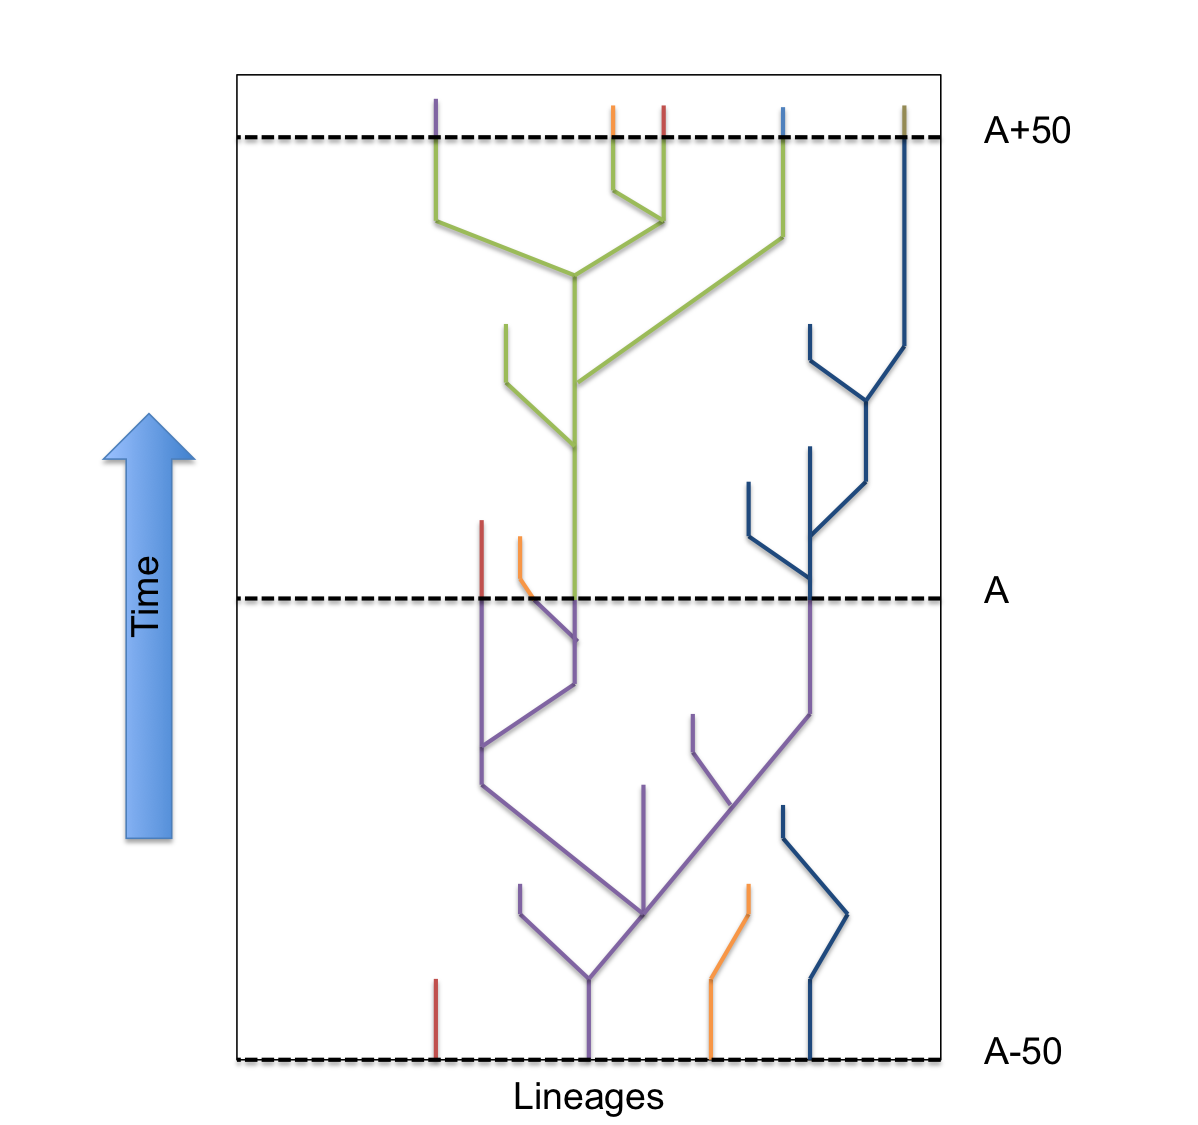
\includegraphics[width=3.5in]{figs/LineageFigure.png}
\caption{\textbf{An illustrative example of how we filter genomes for persistent lineages.} Here, we are using $t = 50$. At time point A, the purple lineage has proven to be persistent and therefore the original genome from A-50 will be considered meaningful. Similarly, the green and blue lineages persist to time point A+50 and so the original green and blue genomes will be considered meaningful as they existed at time point A.}
\label{lineages}
\end{figure}

\subsubsection{Determining boundedness}

In the design of these metrics, we have primarily focused on determining the effect that small changes to a system have on the extent to which that system exhibits hallmarks. However, they can also be used to classify systems in much the same way that evolutionary activity statistics do. As described in Table \ref{eastats}, this classification requires determining whether diversity is increasing without bound. In addition, it would be informative to determine whether complexity is growing without bound. In previous work, the definition of boundedness in this context has been stated in terms of the limit of the suprememum of diversity as time goes to infinity \citep{bedau_classification_1998}. While this is an excellent theoretical definition, taking limits of empirical data as time goes to infinity is generally not practical. Most previous applications of evolutionary activity statistics seem to have determined boundedness based on whether or not a line on a graph appears to be plateauing. This technique has the potential to be misleading \citep{wiser_boundedness_2018}.

Instead, we advocate the use of statistics to determine what mathematical model best fits the observed data. We can then classify the pattern as bounded or unbounded based on the limit of the best-fitting mathematical model. Such an approach has previously been used to demonstrate that fitness is following an unbounded growth pattern in a long-term wet lab evolution experiment with \textit{E. coli} \citep{wiser_long-term_2013, lenski_sustained_2015}.

\subsection{MODES Metrics}

\subsubsection{Change Metric}
Our first metric focuses on whether the genetic makeup of the population is changing in a non-trivial way. This metric will be above zero %, unless the population has converged and no beneficial variation is being introduced.
during adaptive evolution, including situations where the population is returning to previous states due to environmental cycling.
In this work presented here, we use a persistence filter (explained above) to ensure that we mark a genome as new %compared to the previous time point
only if its lineage 
%has persisted for one 
%will persist until the next
went on to persist for a
full $t$ generations, however a different filtering technique (e.g. a shadow run) could be used instead. For this comparison, we first find the genomes from persistent lineages from generation A by determining which genomes have descendants in generation A + $t$. In the example shown in Figure~\ref{lineages}, the genomes at the roots of the green and blue lineages would count as persistent. We then compare these genomes to those found to have been from persistent lineages in the previous time point (e.g. we would compare the roots of the blue and green lineages to the root of the purple lineage in Figure~\ref{lineages}). In this way, we create a sliding window to observe change in the population. Note that the example in the figure assumes the resolution at which data are collected (i.e. the number of generations between time points) is equivalent to the value of $t$, but this does not need to be the case. It may be desirable to have a very long length of $t$ but still gather data frequently. In such a case, each time point is individually filtered by looking ahead $t$ generations, but change is calculated by comparing the set of persistent taxa in the current time point to the set of persistent taxa in the previous time point. 

While there is no change metric in the original conception of evolutionary activity statistics, we expect that it will provide similar information to cumulative evolutionary activity \citep{bedau_comparison_1997}. Change must be positive in systems exhibiting class 3 or higher evolutionary dynamics, as these systems must all exhibit positive novelty. Class 1 systems may or may not exhibit change; an evolving system that stagnates (e.g. many genetic algorithms) would have zero change, whereas a completely neutral system where all change was caused by drift would sometimes have a non-zero amount of change (depending on the value of $t$). Class 2 systems would have non-zero change if they were cycling between fixed states, but not if they were purely the result of stabilizing selection.

\subsubsection{Novelty Metric}
The novelty metric measures how many genomes have evolved in the population that have never been seen previously in the experiment. For this metric we again filter out genomes that do not have descendants in $t$ generations, enabling us to focus on meaningful novelty. As with change, we could have used a different filtering technique instead. To measure novelty, we simply count how many genomes from persistent lineages have never been in a previous time point’s persistent genome pool. It is possible with this metric for a genome to evolve, but not persist, and therefore not be recorded in the permanent history, but then evolve and persist at a later point and be counted as novel. Once a genome has been counted as novel, however, it is part of the permanent history and will never be counted in the novelty metric again. Thus, while a genome could be delayed in being counted as novel, or not counted if it never persists, it will not be counted twice. Our novelty metric is functionally equivalent to $A_{new}$ in evolutionary activity statistics \citep{bedau_comparison_1997}.    

\subsubsection{Complexity Metric}
The complexity metric measures the maximum complexity (informative sites) of any organism found in the entire population. We recommend the approach described in the section on  ``Identifying meaningful sites in genomes'' above. Once the meaningful sites have been identified, they can be counted to get a measurement of complexity; the value of the complexity metric at a given time point is the highest observed count of informative sites across all taxa in the population that make it through the filter. Further, complexity can be measured even more accurately by using information-theoretic techniques where all possible mutations are considered at each site, and ideally some epistatic interactions.

There is no equivalent to the complexity metric in evolutionary activity statistics. However, as many believe growth in complexity to be an important hallmark of open-ended evolution \citep{taylor_open-ended_2016}, we feel it is a critical addition. In particular, it would be interesting to find non-trivial systems that exhibit unbounded growth in complexity. We suspect that such growth could only occur in systems exhibiting class 4b or 4c evolutionary dynamics, as bounded evolutionary activity should imply bounded complexity (although the converse is not true).

\subsubsection{Ecological Metric}
The ecological metric measures the amount of information in the population as a whole. While organisms may not contain increasing amounts of information in their individual genomes (as measured by the complexity metric), they could still be increasingly diverse and therefore contain increased information collectively in the population. Ideally, we would measure this collective information by tracking the origin of each piece of information across all genomes in the population and summing up the number of unique pieces of information. Unfortunately, this approach is not computationally practical for many systems. As a proxy, we can look at the diversity of post-filter genotypes reduced to informative sites. Complex ecologies in which multiple subsets of the population are using different information about the environment to survive are likely to be characterized by a relatively balanced distribution of individuals across the various successful phenotypes. Thus, we use Shannon entropy, a popular metric of diversity that also measures evenness, to measure the diversity of the persistent genotypes and calculate the ecological metric. This metric is equivalent to $D$ in evolutionary activity statistics \citep{bedau_comparison_1997}, assuming we chose genotypes reduced to informative sites as components.

\section{Experimental Systems}

We used two radically different experimental systems in order to ensure both that these metrics can be broadly applied and that they produce meaningfully consistent results.

\subsection{NK Landscape}
To begin a systematic examination of MODES metrics, we used a simple NK model~\citep{kauffman_towards_1987}. An NK model uses two parameters, N and K, to randomly generate a fitness landscape. N specifies the number of sites in the genome, each of which is a 0 or a 1. The fitness landscape specifies the effect of a given value at a given site on the fitness of the bit-string organism. This fitness effect depends on the values at the K subsequent adjacent sites. As such, K tunes the ruggedness of the landscape; low values of K produce smooth landscapes with few peaks, whereas high values produce landscapes with many peaks. We chose to use NK models because they are a well-understood system for studying general questions about evolutionary dynamics.

\subsubsection{Experimental Treatments}
Our basic treatment used $N=20$ (i.e., 20 bits in an individual) and $K=3$ (the fitness contribution of each bit was influenced by three other bits).  We used a population size of 200 and a mutation rate of three sites per birth (three bits were randomized in each birth, so there is a 1/8 probability of all three retaining their original values), with tournament selection and a tournament size of 15.
In addition to this baseline
treatment, we performed eight experimental treatments: \textbf{High K} tests the effect of a highly rugged landscape (K=10) where fitness is effectively randomized whenever a mutation occurs.  \textbf{High N} tests the effect of longer bit-string genomes (N=100), allowing for a higher potential complexity.  \textbf{Low Mut} and \textbf{High Mut} test the effects of more extreme mutation rates (1 bit and 6 bit randomizations per birth, respectively); we expect the mutation rate to be important for finding new areas of the fitness landscape and thus our novelty metric.  \textbf{Small Pop} and \textbf{Large Pop} vary the population size (to 20 and 1000 respectively); in small populations we expect more drift in the population, allowing more change, while in a large population we expect stronger selection and consequently that a higher percentage of changes along the line of descent are beneficial.  Finally, we included two special treatments: in \textbf{Changing Environments}, the fitness function was toggled every 500 generations, allowing us to see the effect of changing selective pressures where the populations was not able to stay on a single peak.  In \textbf{Fitness Sharing} organisms that were too similar to each other detracted from each other's fitness, creating a pressure to explore multiple portions of the landscape at the same time and, ideally, maintain a high diversity  \citep{goldberg_genetic_1987}.

\subsection{Avida}

The Avida Digital Evolution platform is a popular artificial life system for studying evolutionary dynamics \citep{ofria_avida:_2004}. Avida consists of a population of self-replicating digital organisms with circular genomes composed of assembly-code-like instructions. Over the course of their lifetimes, organisms in Avida execute the code in their genome. The population is initially seeded with a single hand-coded organism that inefficiently copies itself and does nothing else. Each organism lives in its own cell in a toroidal grid. When an organism copies itself, its offspring is placed in a different cell, overwriting any previous occupant of that cell. Thus, there is pressure for individuals to reproduce quickly, before others copy over them. During the replication process, mutations are probabilistically introduced. Thus, the system contains inheritance, variation, and selection, causing evolution by natural selection to occur. Optionally, ``tasks'' can be added to the environment in Avida. These are computational problems that organisms can perform for a reward in the form of additional CPU cycles that allow organisms to execute their code faster.

\subsubsection{Experimental Treatments}
To understand how MODES metrics will behave in a full-featured artificial life system, we tested them in Avida under a variety of scenarios. For all experiments, we used a well-mixed population in order to speed up the expected rate of coalescence. All other parameters in Avida were left at their default values. We ran experiments in two different environments. The \textbf{empty} environment has no tasks - all evolution is focused entirely on optimizing the efficiency with which organisms can self-replicate. The \textbf{logic-9} environment, which has been used in many prior experiments (e.g. \citep{lenski_evolutionary_2003}), contains tasks for all one- and two-input boolean logic functions.

Artificial life systems necessarily have constraints on the amount of time and memory we can give them. It is important in open-ended evolution research to determine whether these constraints are imposing practical limitations on the dynamics the system exhibits \citep{zaman_investigating_2018}. To do so, we ran experiments in each environment at three different population sizes: 500, 1000, and 2000. In each condition, we ran 30 replicate runs of Avida.

Additionally, to understand how sensitive our metrics are to the choice of the filter length ($t$) we conducted some additional experiments in the empty environment in which we varied $t$. At each of the three population sizes, we tried $t$ values of 500, 1000, and 2000. To ensure that we always have data from a filter length larger than population size, we also included a condition with a population size of 2000 and a $t$ of 4000.

\subsection{Implementation Details}
If not implemented with care, these metrics can become computationally intractable in the context of the long experiments that open-ended evolution research often entails. In particular, RAM requirements can become prohibitive. We provide a few high-level approaches to mitigating these issues.

The largest memory cost is imposed by the novelty metric's requirement that we keep track of every taxon that has ever passed the persistence filter. Because we only need to know when we encounter a repeat taxon (rather than storing an archive of all taxa we have encountered), we can dramatically reduce this cost by using a Bloom filter \citep{Bloom:1970:STH:362686.362692}. Although this approach does introduce a (tunable) risk of false negatives (i.e. miss-classifying a novel taxon as not novel), this risk only makes the metrics more conservative. 

The next largest cost is imposed by needing to keep track of the phylogeny over time. In addition to standard phylogenetic pruning techniques (such as removing all taxa that do not have extant descendants), we can safely remove all taxa that died before the current generation minus $t$\footnote{An important caveat is that this approach will only work with a strictly increasing unit of time. In many systems (including Avida) the average generation is not guaranteed to consistently increase. To support such systems, our implementation of the metrics allows for time to be tracked using two units at once, one corresponding to generation, and one that is guaranteed to be strictly increasing.}. This optimization prevents the tree from growing without bound over the course of the experiment.

Lastly, it is helpful to be aware that increasing $t$ will reduce computational demands by increasing the percentage of taxa that will be filtered out. With these optimizations, MODES metrics can be implemented with minimal overhead.

\subsection{Code Availability}
A C++ implementation of MODES is available as part of the Empirical library \citep{charles_ofria_2018_1439475}. The library is header only, and designed to be as easy to integrate into existing systems as possible. As a proof of this concept, the Avida experiments presented in this paper were carried out using a lightly modified version of Avida that incorporated this implementation of our metrics \citep{david_bryson_2018_1439479}. All analyses and statistics for this paper were conduction used the R Statistical Computing Language \citep{r_core_team_r:_2017} and the ggplot2 plotting library \citep{wickham_ggplot2_2016}. All code used in this paper is open source and freely available [CITE].


\section{Results and Discussion}
To ensure that these metrics are capturing the dynamics that we want them to, we tested them on a range of variants of our basic NK model and a range of conditions in Avida. The preliminary results for each metric are presented here.

\subsection{Change Metric}
%For a system to exhibit open-ended evolution, it is clearly necessary for the composition of the population to be changing in some meaningful way, although this change needn't always be novel. We measured the meaningful change in our systems under varying environmental conditions to confirm that this metric responds intuitively. 
In the baseline and low mutation rate conditions for the NK Landscape, change is close to 0 (see Figures~\ref{change_time} and \ref{change}), indicating that our metrics are capable of detecting the stagnation typical of many genetic algorithms. As shown in Figure~\ref{change_time}, several environmental changes increase the amount of meaningful change found in the NK Landscape populations over time. When organisms are forced to share fitness between others with the same genotype, the amount of change increases and remains higher than the baseline over time. Conversely, when the environment changes frequently, there is an initial spike of increased change that quickly drops back down to the baseline value.

\begin{figure}
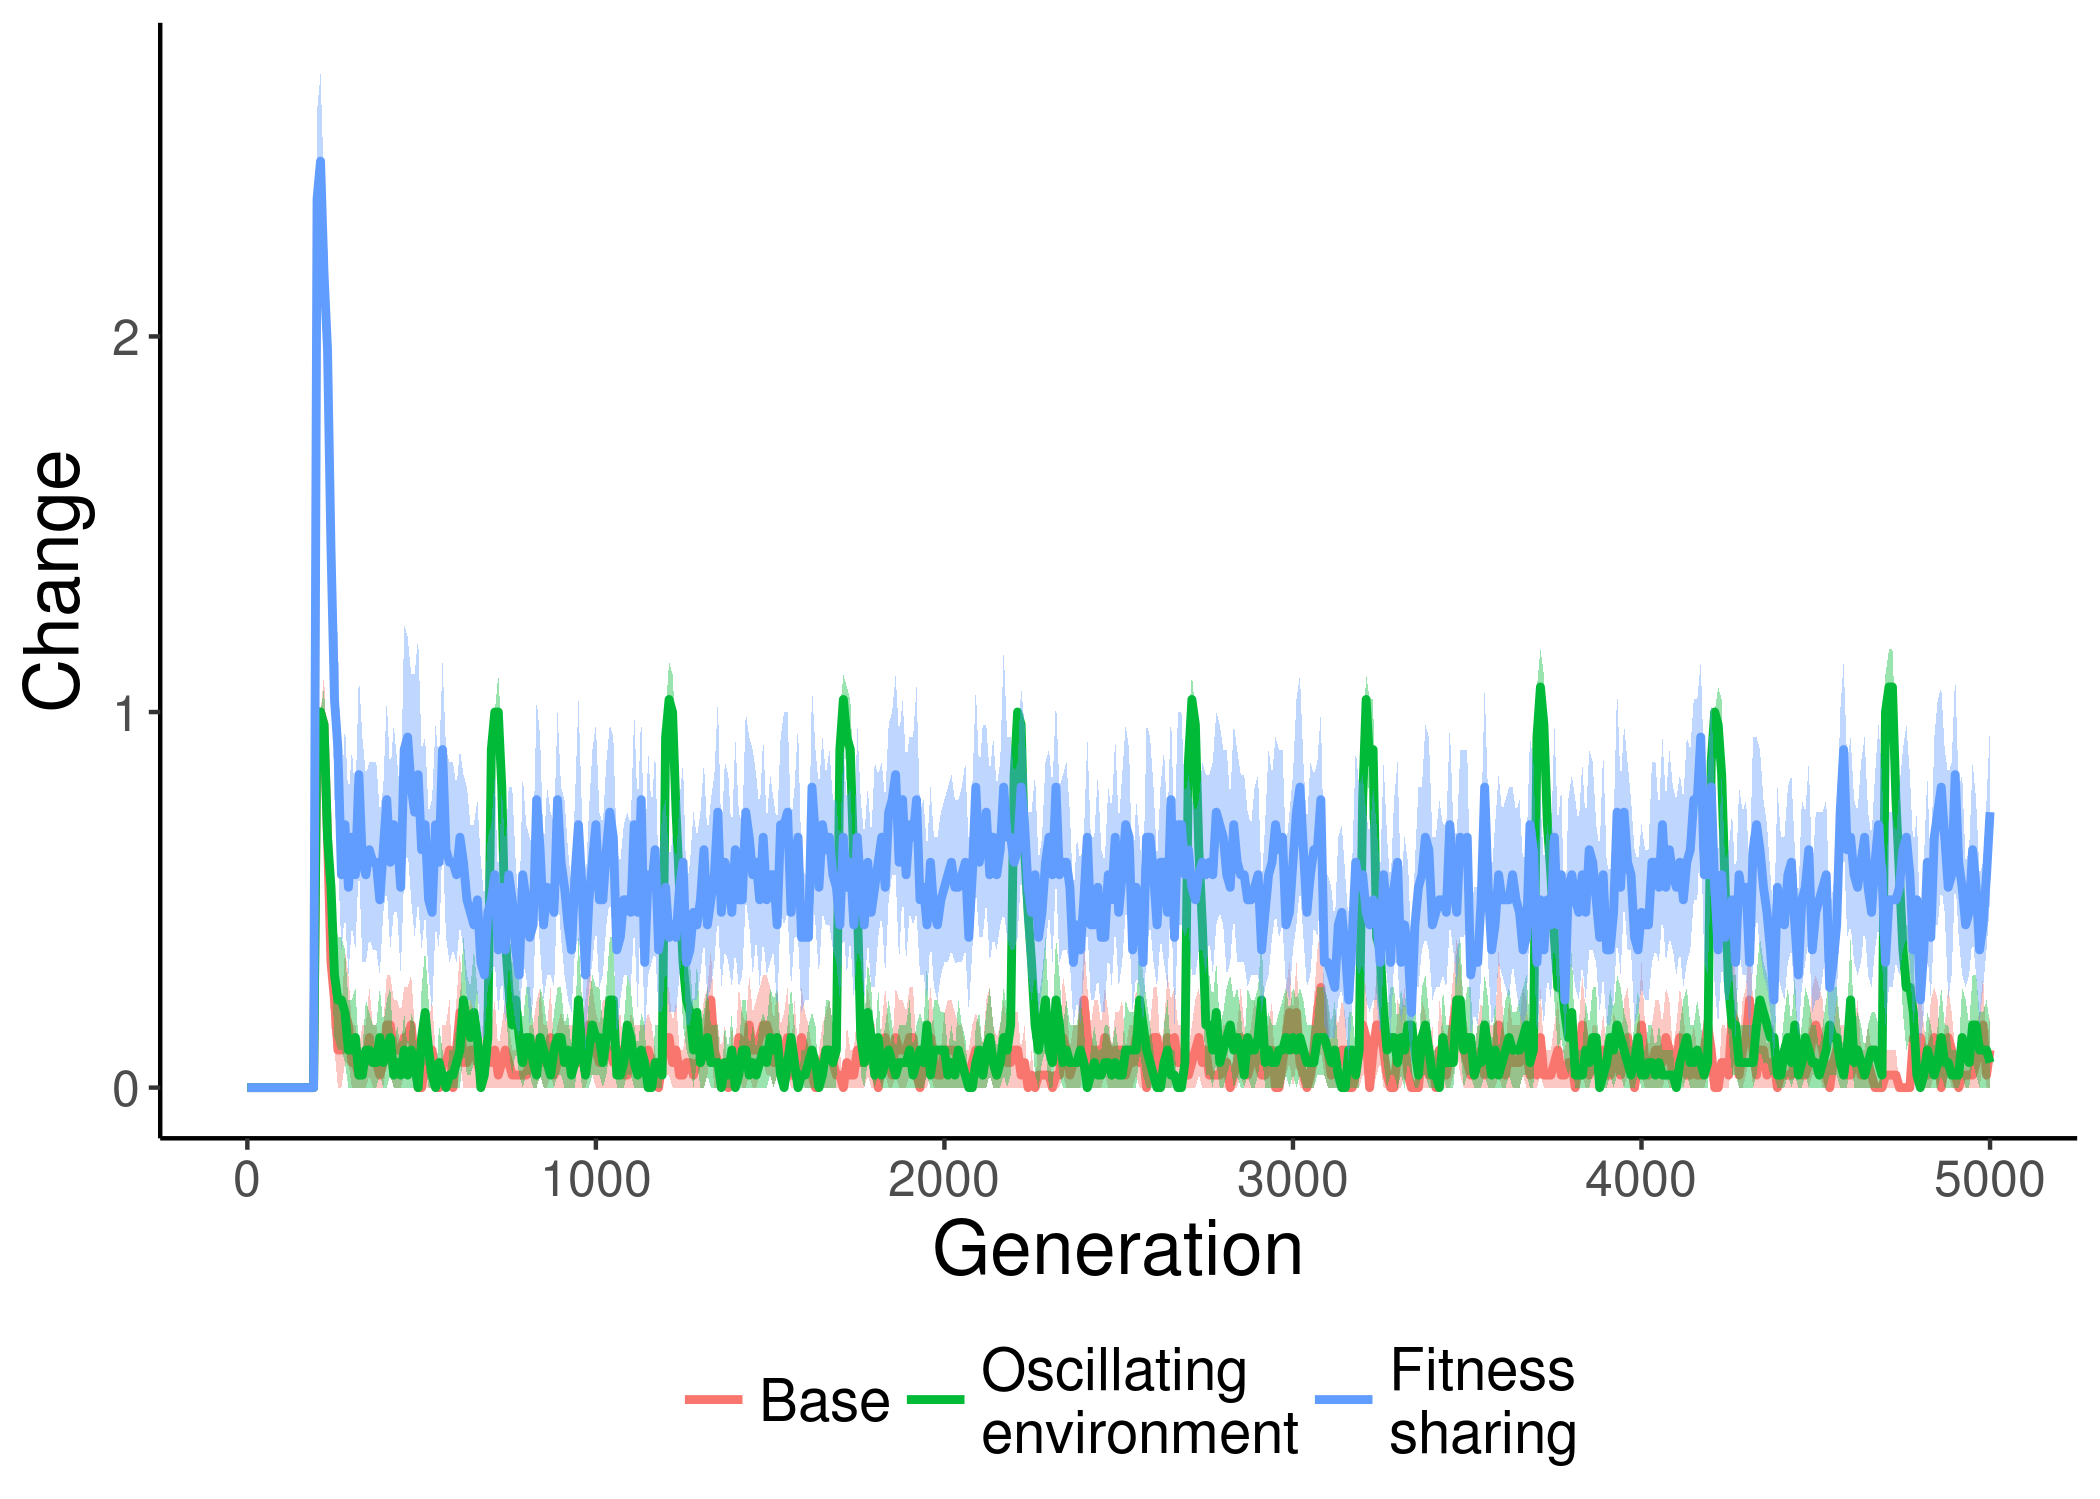
\includegraphics[width=3.5in]{figs/change_changing_environments.png}
\caption{\textbf{Amount of change at over time in varying NK Landscape environments.} As measured by the change metric, fitness sharing increases the amount of change in the population over time. Conversely, a routinely changing environment leads to spikes in change that quickly drop as the population converges again. Shaded region represents a bootstrapped 95\% confidence interval around the mean.}
\label{change_time}
\end{figure}

\begin{figure}
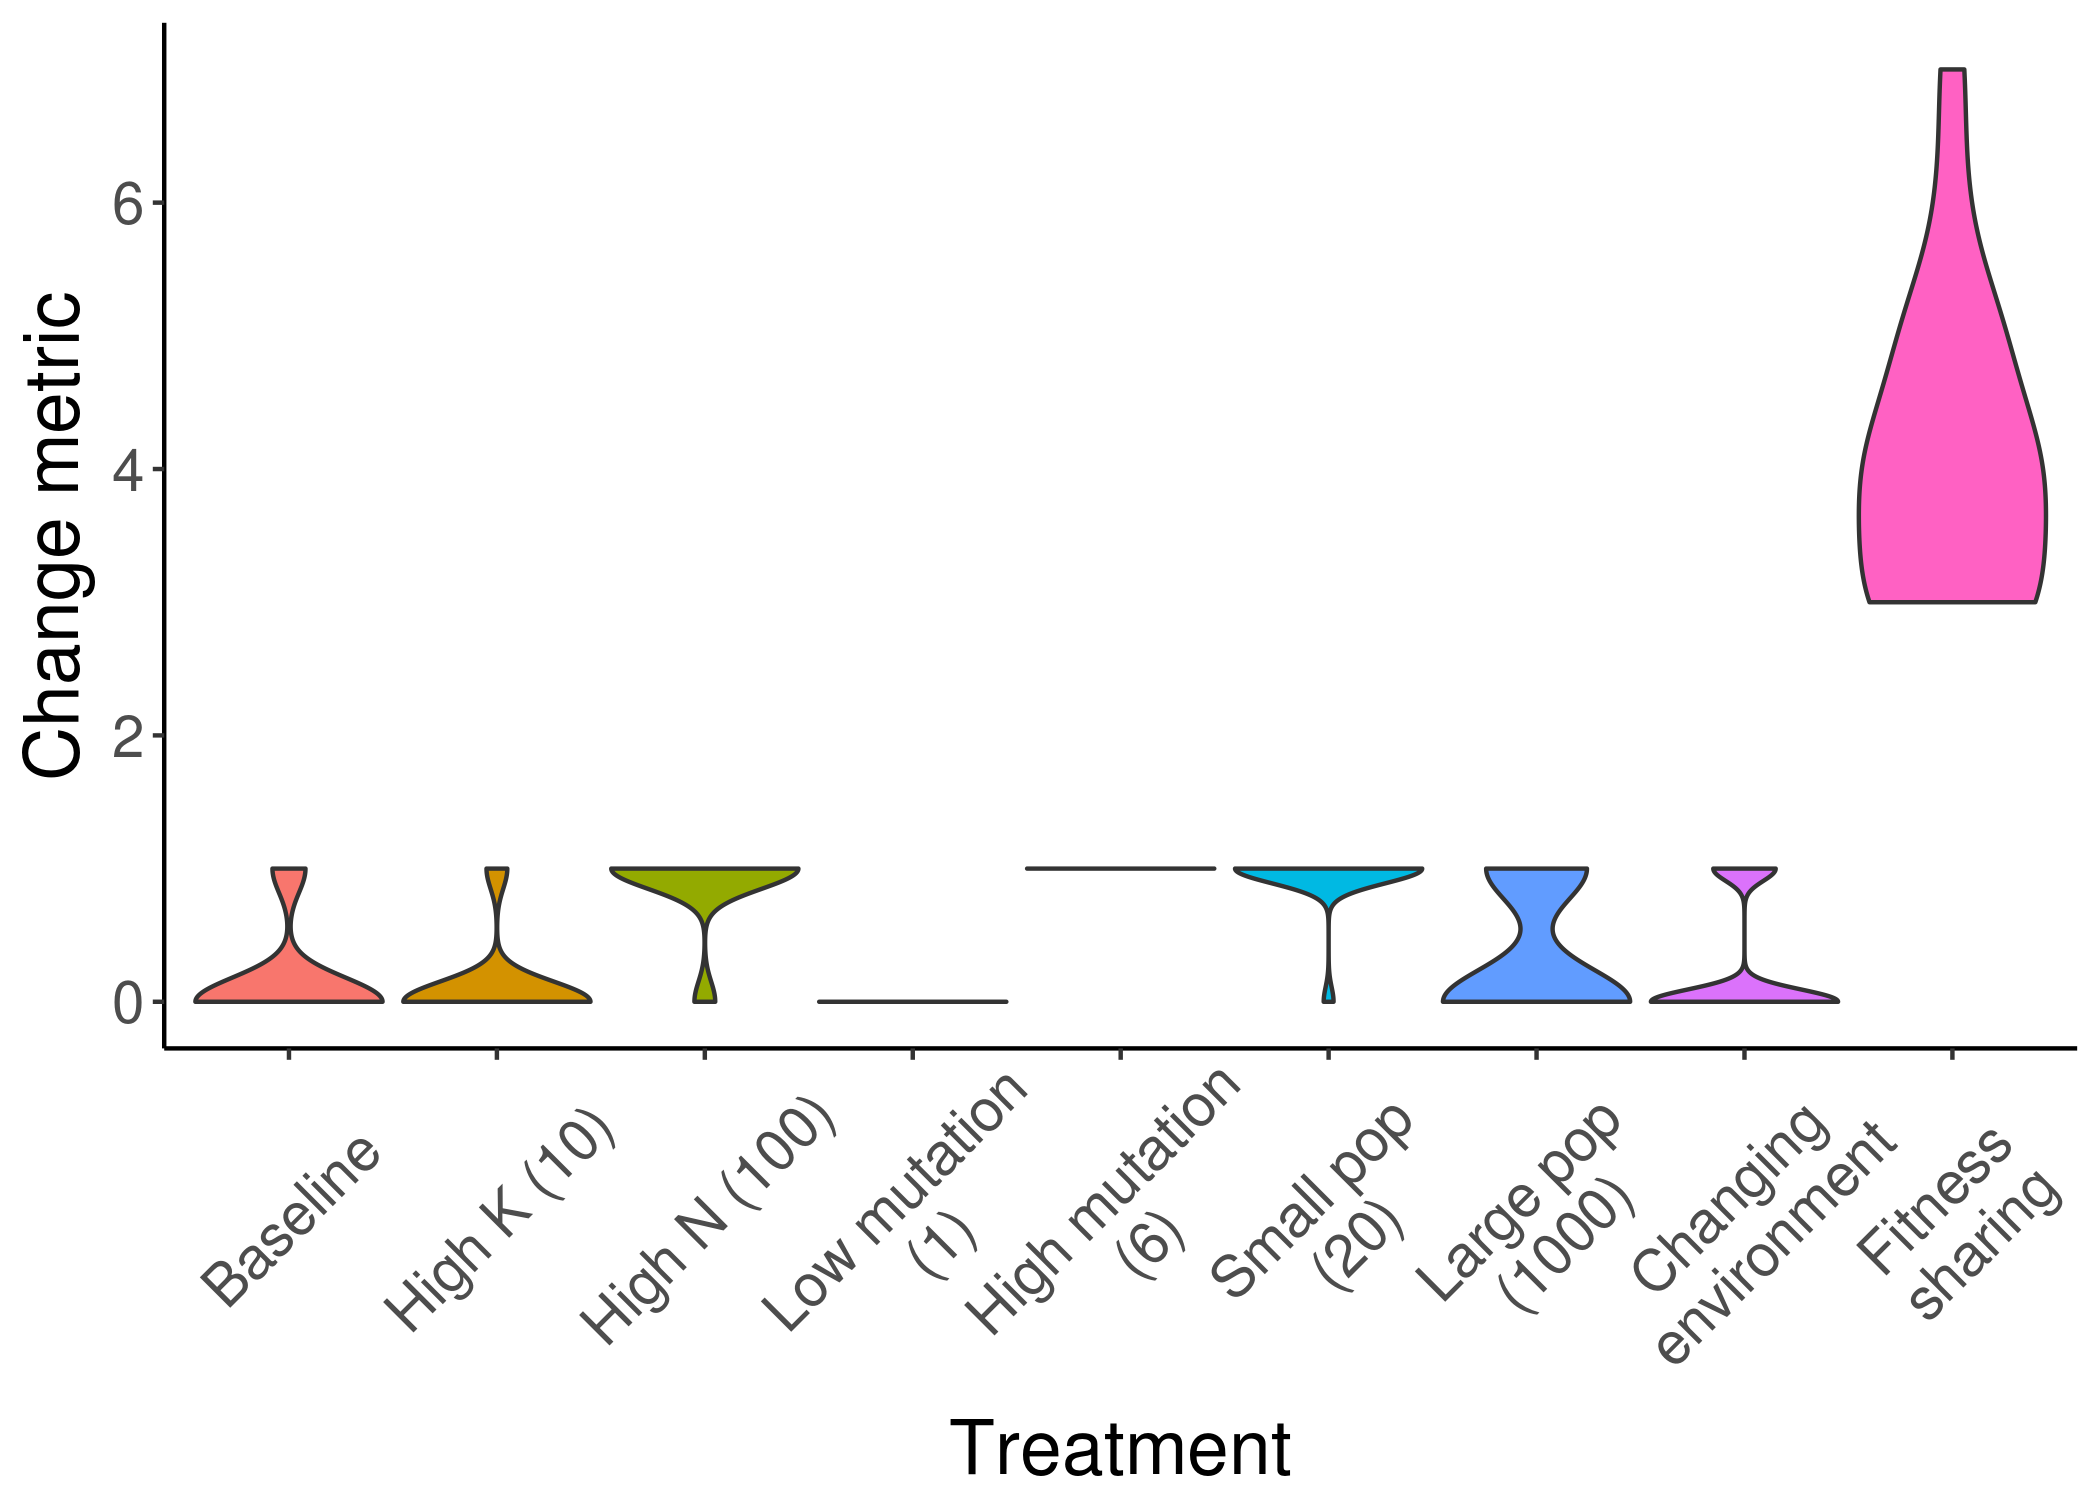
\includegraphics[width=3.5in]{figs/changeboxplots.png}
\caption{\textbf{Amount of change at final generation in varying NK Landscape environments.} As measured by the change metric, environmental conditions that increase the amount of change at the final time point include: increasing the size of the genome (N), increasing the mutation rate, decreasing the population size, and implementing fitness sharing. Shaded region represents a bootstrapped 95\% confidence interval around the mean.}
\label{change}
\end{figure}


The majority of environmental conditions we tested in the NK Landscape system produced dynamics over time qualitatively similar to the baseline treatment. In Figure~\ref{change} we show the amount of meaningful change in populations at the final time point in more environmental conditions. Larger genomes (N) lead to increased meaningful change because they allow for a larger search space that the population can continuously mutate within, leading to more beneficial mutants. A higher mutation rate leads to increased meaningful change because mutations are necessary to create any meaningful change in this system. A smaller population size produces more meaningful change because a small population cannot hold as many different genomes at one time and therefore there are more genomes that can arise that are different than what is in the previous population. Finally, fitness sharing produces increased meaningful change because it creates a constant pressure for the population to adapt away from whatever is the current dominant genotype.

\begin{figure}
    \centering
    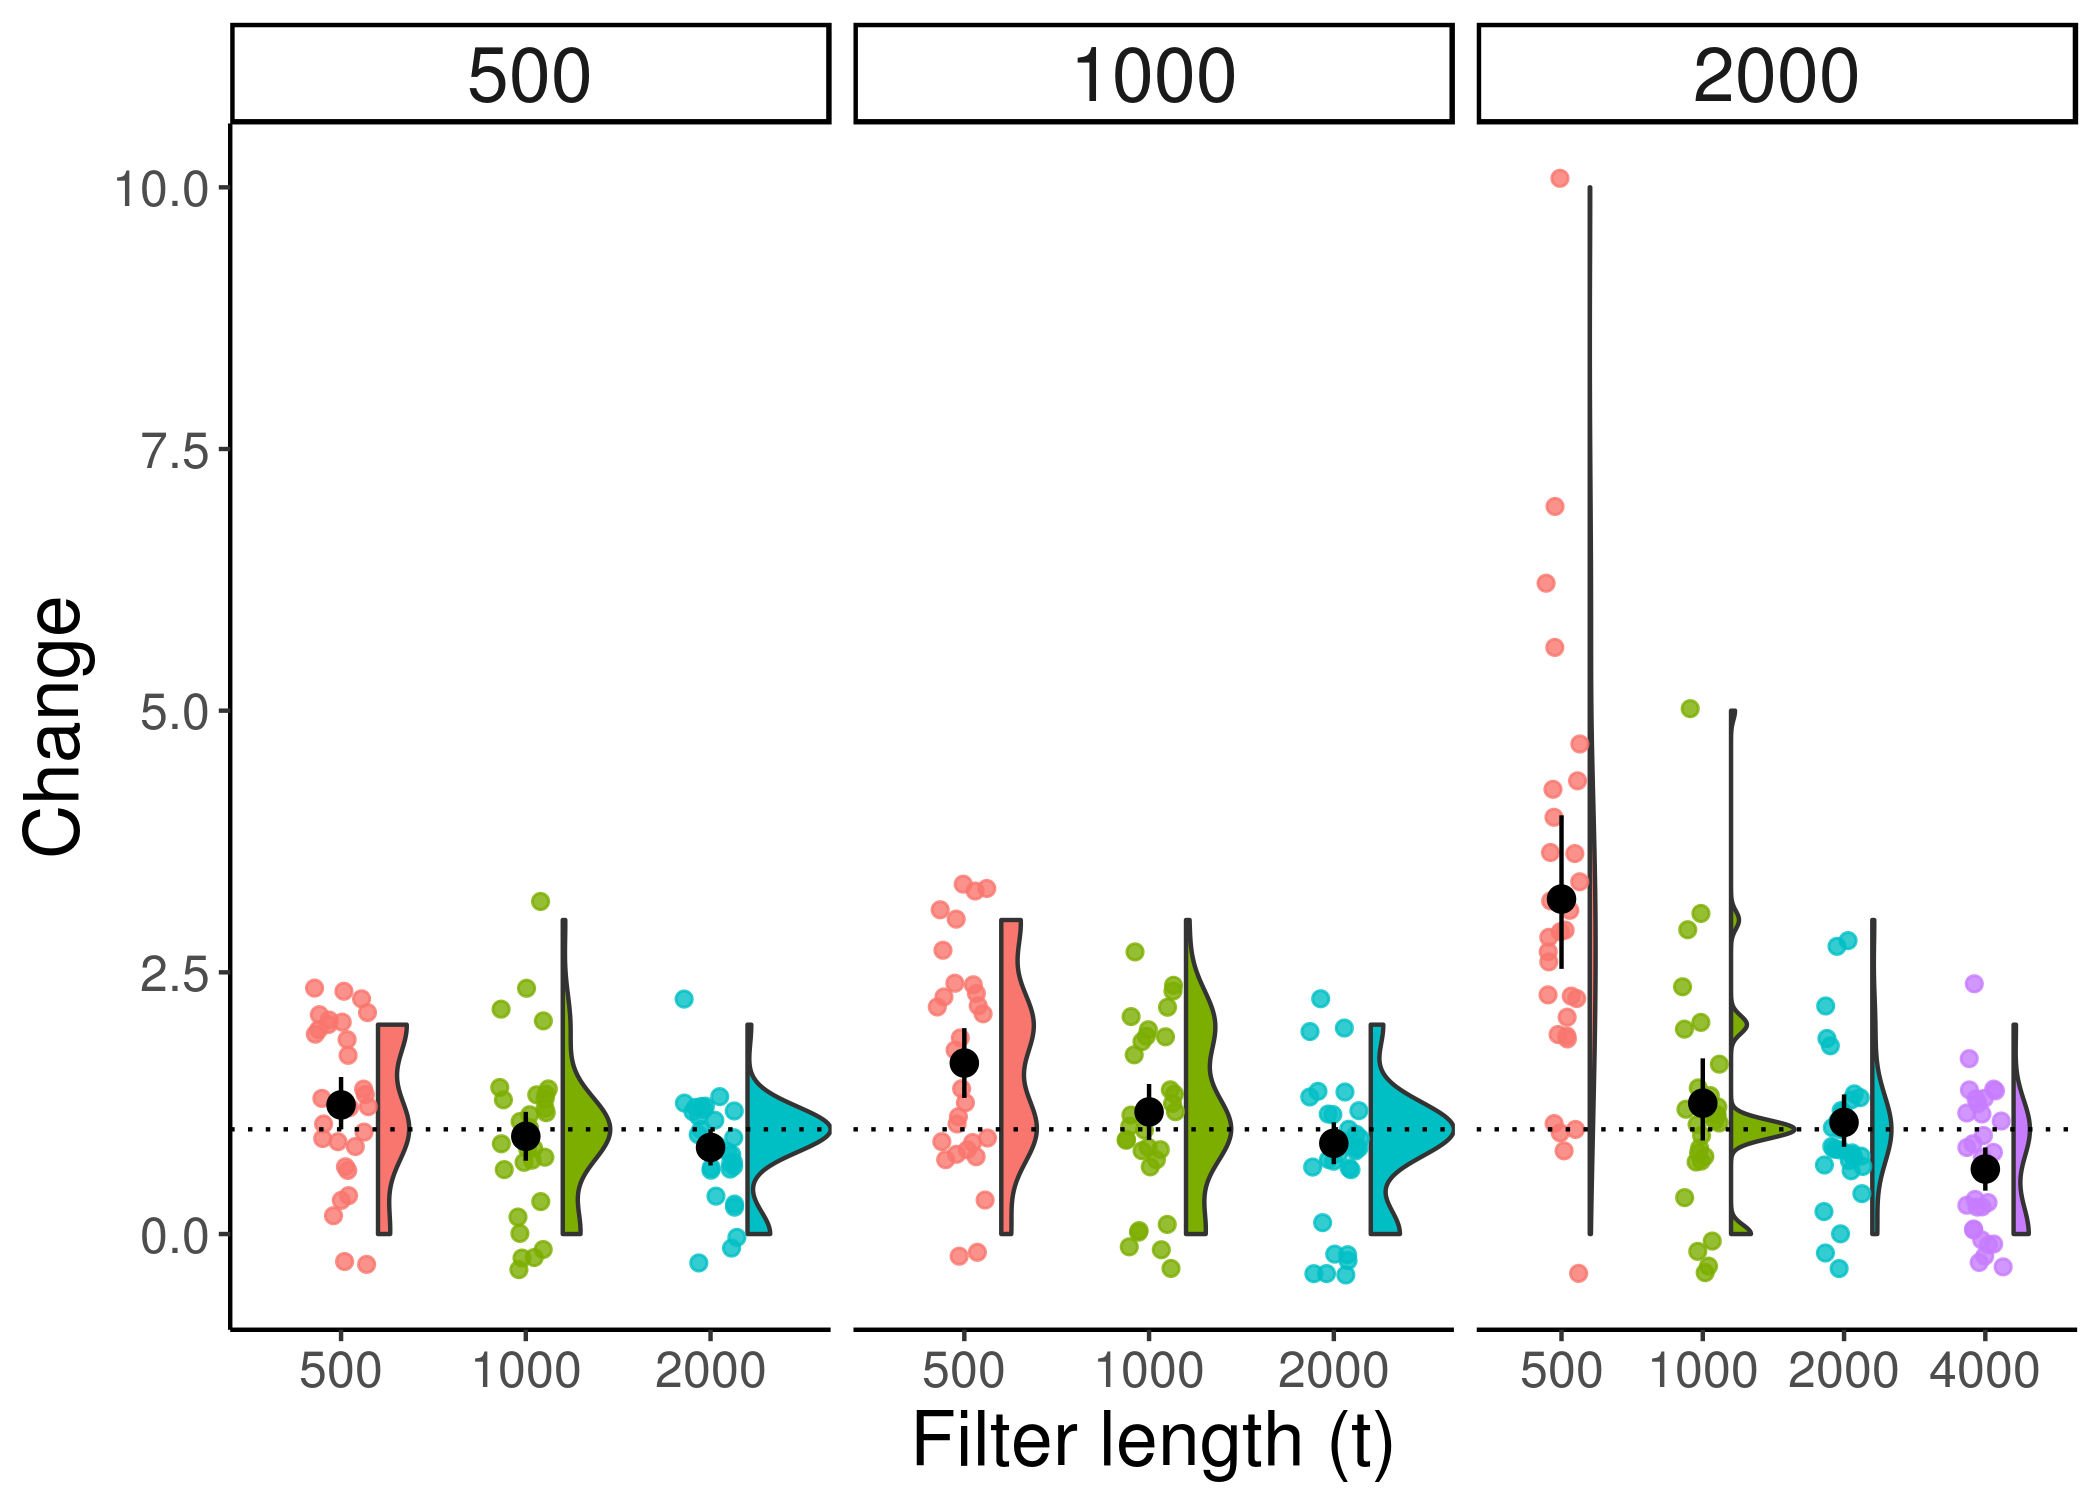
\includegraphics[width=3.5in]{figs/avida_filter_change_end.png}
    \caption{\textbf{Rain-cloud plot of change in Avida at generation 200,000, across multiple population sizes and filter lengths.} Labels along the top indicate population size. Black circle and lines indicate mean and bootstrapped 95\% confidence interval. For more information on rain-cloud plots, see \citep{allen_raincloud_2018}.}
    \label{fig:avida_filter_change}
\end{figure}

In Avida, there is always at least a little change (see Figure \ref{fig:avida_filter_change}. This observation is consistent with previous findings that fitness in Avida increases indefinitely \citep{wiser_analysis_2015}, as an increase in fitness implies both change and novelty. Based on coalescence theory, we would expect change in the empty environment to usually be less than or equal to one, because it is a single-niche environment. During every interval, either a fitter genotype will arise and sweep the population or the current fittest genotype will remain dominant. Because our value of $t$ is not higher than the maximum possible coalescence interval, we should also expect to see the occasional time point with change greater than one. Our data are roughly consistent with this expectation. In addition, there is a subtle downward trend in the change data, likely due to the progressively increasing difficulty of finding beneficial mutations.

As expected, increasing the filter length, $t$, decreases the amount of change observed because fewer taxa are able to get through the filter (see Figure \ref{fig:avida_filter_change}). In general, using a value of $t$ equal to population size seems to be an adequate filter. The confidence interval for the mean of these conditions always overlaps with 1, indicating that a substantial amount of filtering is occurring. Using lower values of $t$ begins to lead to substantial increases in the variance of observed change. Using a higher value of $t$ does further reduce noise, but with diminishing returns. In the empty environment, population size does not appear to have much impact on change, implying (unsurprisingly) that population size does not exert pressure on evolutionary dynamics in this environment.

\begin{figure}
    \centering
    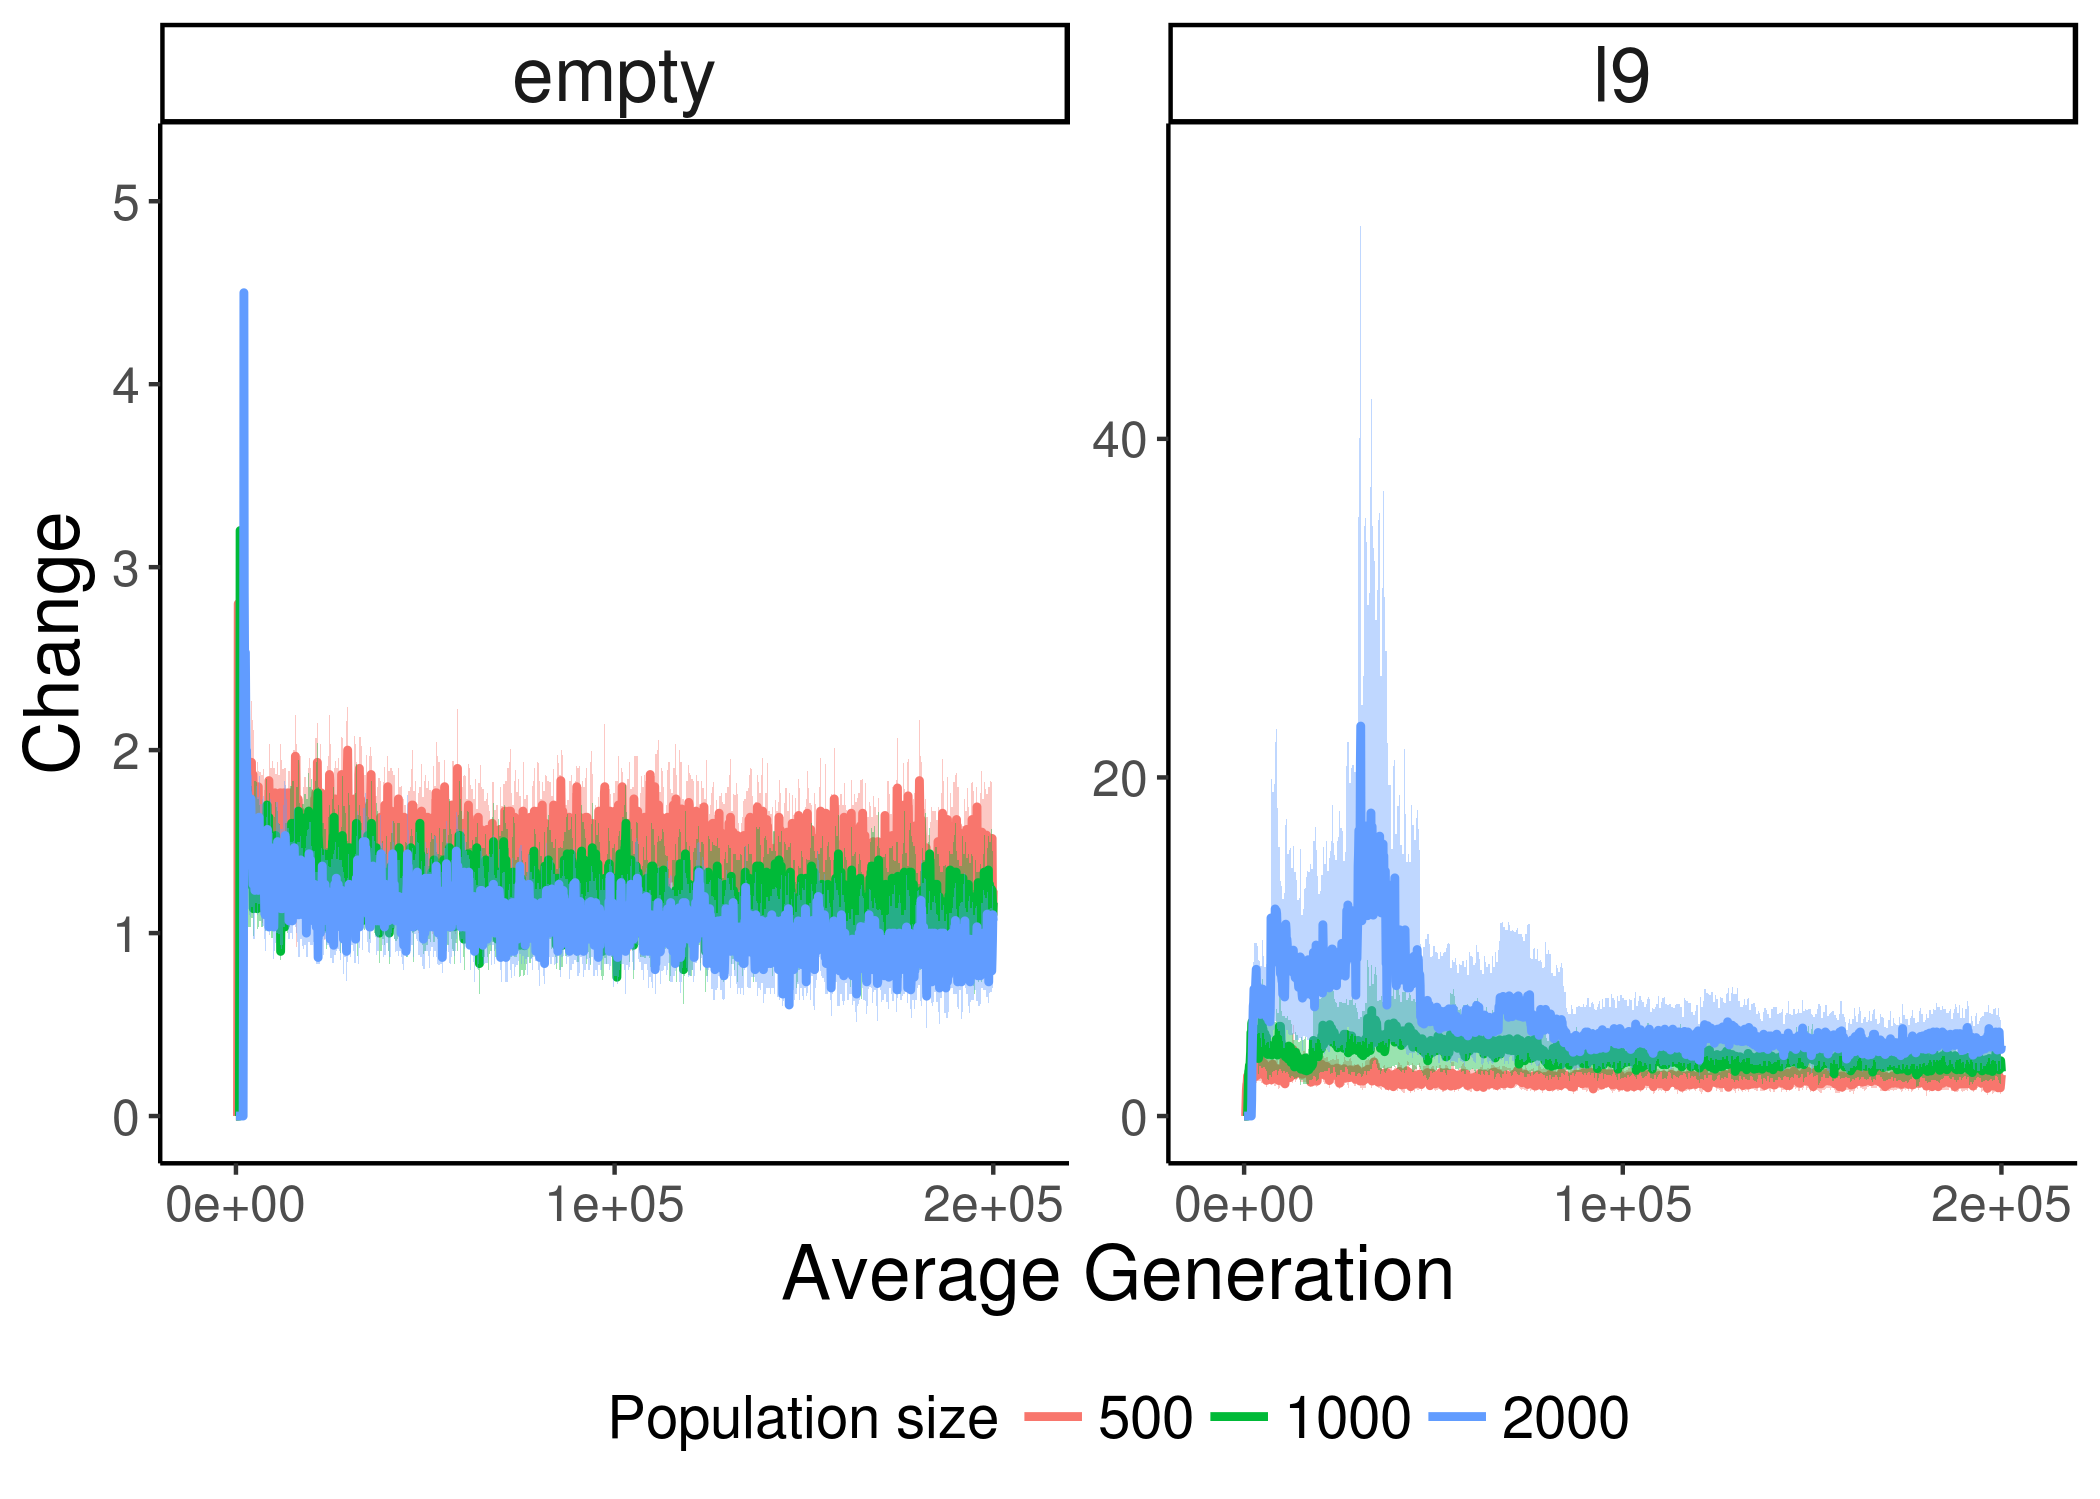
\includegraphics[width=3.5in]{figs/avida_env_change.png}
    \caption{\textbf{Change over time across different environments and population sizes in Avida.} Note that y axes have different scales.}
    \label{fig:avida_env_change}
\end{figure}

In the logic-9 environment, however, there is a slight increase in change as population size increases, particularly early in the experiment (see Figure \ref{fig:avida_env_change}). Additionally, change is generally a little higher in the logic-9 environment than the empty environment. This distinction is an unexpected benefit of using a value of $t$ too low to guarantee coalescence. Logic-9 is a single-niche environment, so if we chose a large enough value of $t$, we would expect change to always be less than or equal to 0. However, logic-9 is a more complex environment than the empty environment, which increases the odds that multiple lineages will be able to keep evolutionary pace with other for a substantial amount of time. As such, at the values of $t$ we used, our change metric is able to reflect the fact that more is going on in the logic-9 environment than the empty environment. 

While change is a metric often not considered in discussions of open-ended evolution, these results show that the amount of meaningful change can reflect differences in the environment and evolution of the populations and is likely a necessary dynamic for open-ended evolution. Our change metric responds in intuitive ways to variations in parameter settings, suggesting that it is a reliable indicator of the dynamics we designed it to capture. 

\subsection{Novelty Metric}
%The continuous production of meaningfully new genomes is necessary for what is generally considered open-ended evolution, because without meaningfully novel genomes, nothing ``interesting'' can emerge. 
As shown in Fig~\ref{novelty_time}, a higher mutation rate increases the amount of novelty generated by the NK Landscape system. This result is to be expected, because more mutations make it easier to cross fitness valleys and otherwise traverse the fitness landscape. As expected, even at a high mutation rate, novelty does start to decrease over time as the search space is explored.

\begin{figure}
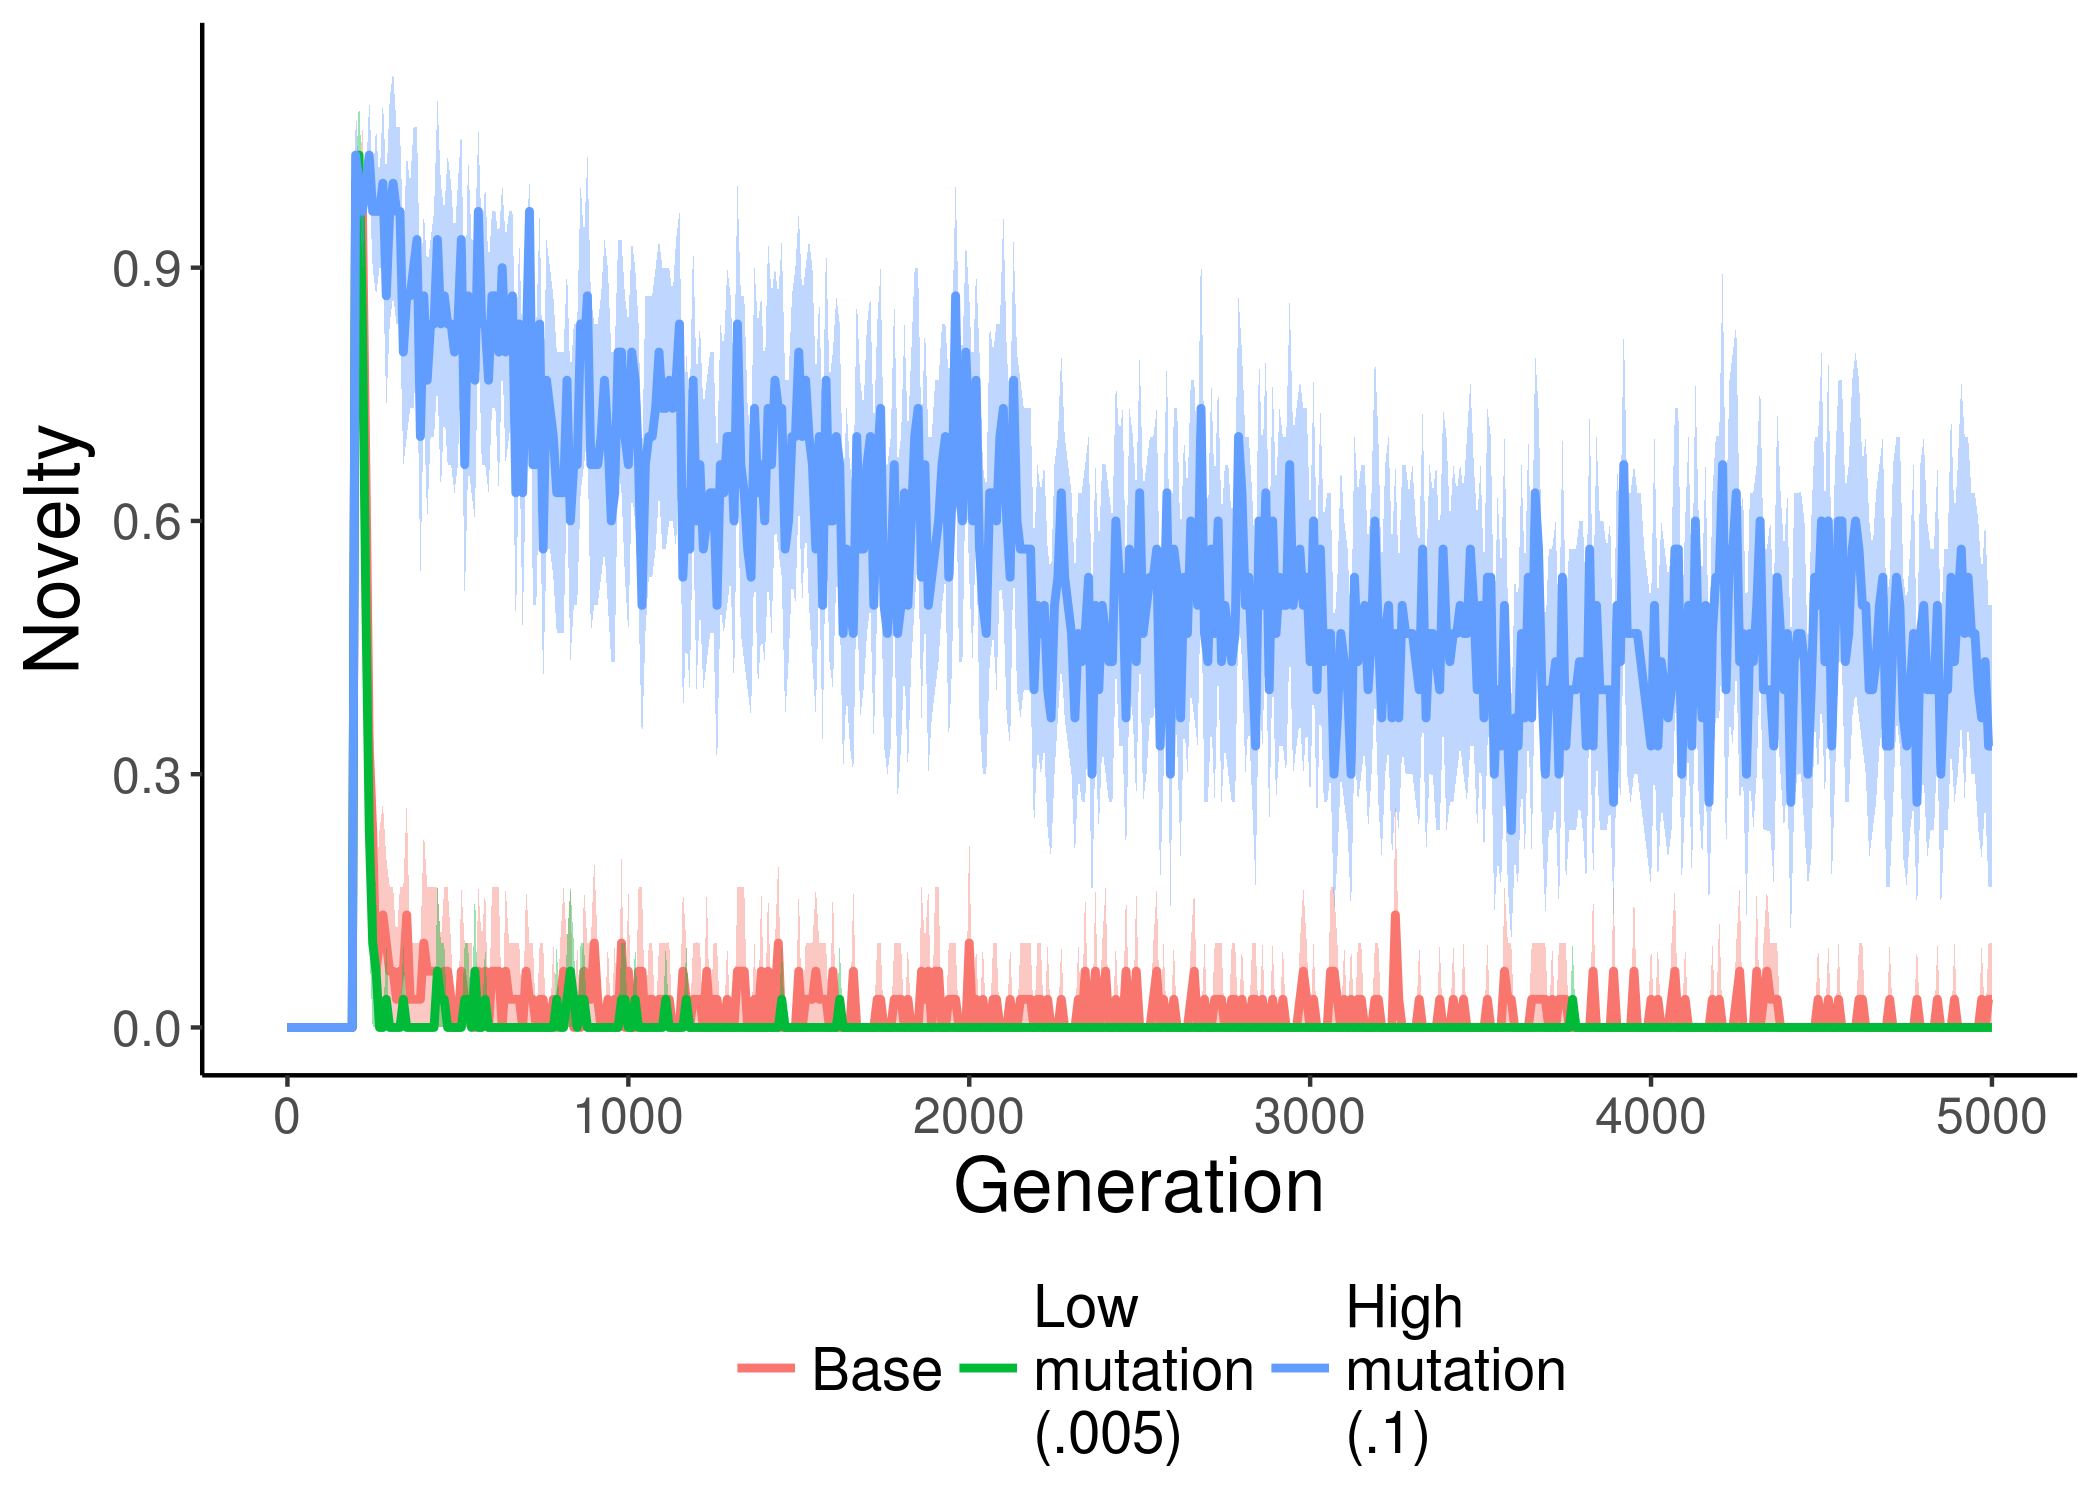
\includegraphics[width=3.5in]{figs/novelty_mean_mut_rate.png}
\caption{\textbf{Amount of novelty over time in NK Landscape with varying mutation rate.} The novelty metric measures the number of completely new meaningful genomes that have lineages that persisted since the previous time point. As the mutation rate increases, more novelty is continuously produced. However, at all mutation rates the novelty decreases over time. Mutation rate 3 is the baseline treatment in previous graphs. Shaded region represents a bootstrapped 95\% confidence interval around the mean.}
\label{novelty_time}
\end{figure}

We again found that the majority of treatments had a qualitatively similar trajectory over time and therefore in Figure~\ref{novelty} we show only the final novelty value. As predicted, the baseline treatment has stopped producing meaningful novelty by the final time point. However, many environments do allow for continuing production of novelty, specifically increased epistasis (K), larger genomes (N), higher mutation rate, differing population size, and fitness sharing. Epistasis increases the value of the novelty metric at the final generation because the population must explore a rugged fitness landscape instead of converging to a single fitness peak, leading to more adaptive novel genomes to discover throughout evolution. Larger genomes allow for more novelty at the final generation because they increase the size of the search space and therefore how many genomes can ever be considered novel. Smaller population sizes increase novelty at the final generation because it takes the population longer to discover many genomes, leaving enough to still be novel at the end of the experiment. Conversely, larger population sizes allow for some increase in novelty over the baseline treatment because the increased number of organisms makes it easier for more of the search space to be explored. Finally, fitness sharing increases the final novelty by creating a selective pressure to explore genotypes that are not currently common in the population; many of these will be novel, as novel genotypes are, by definition, not present in the population.

Like NK Lanscapes, Avida shows gradually declining novelty over time (although novelty in Avida declines more slowly). This trend presumably reflects the declining availability of beneficial mutations. Interestingly, the novelty and change graphs from Avida look almost identical, implying that there is little cycling among previously discovered solutions. This result, too, is consistent with the previously observed indefinite fitness increases in Avida \citep{wiser_analysis_2015} - if the population is always getting fitter, genotypes from earlier in the run would be unlikely to survive in the present.

\begin{figure}
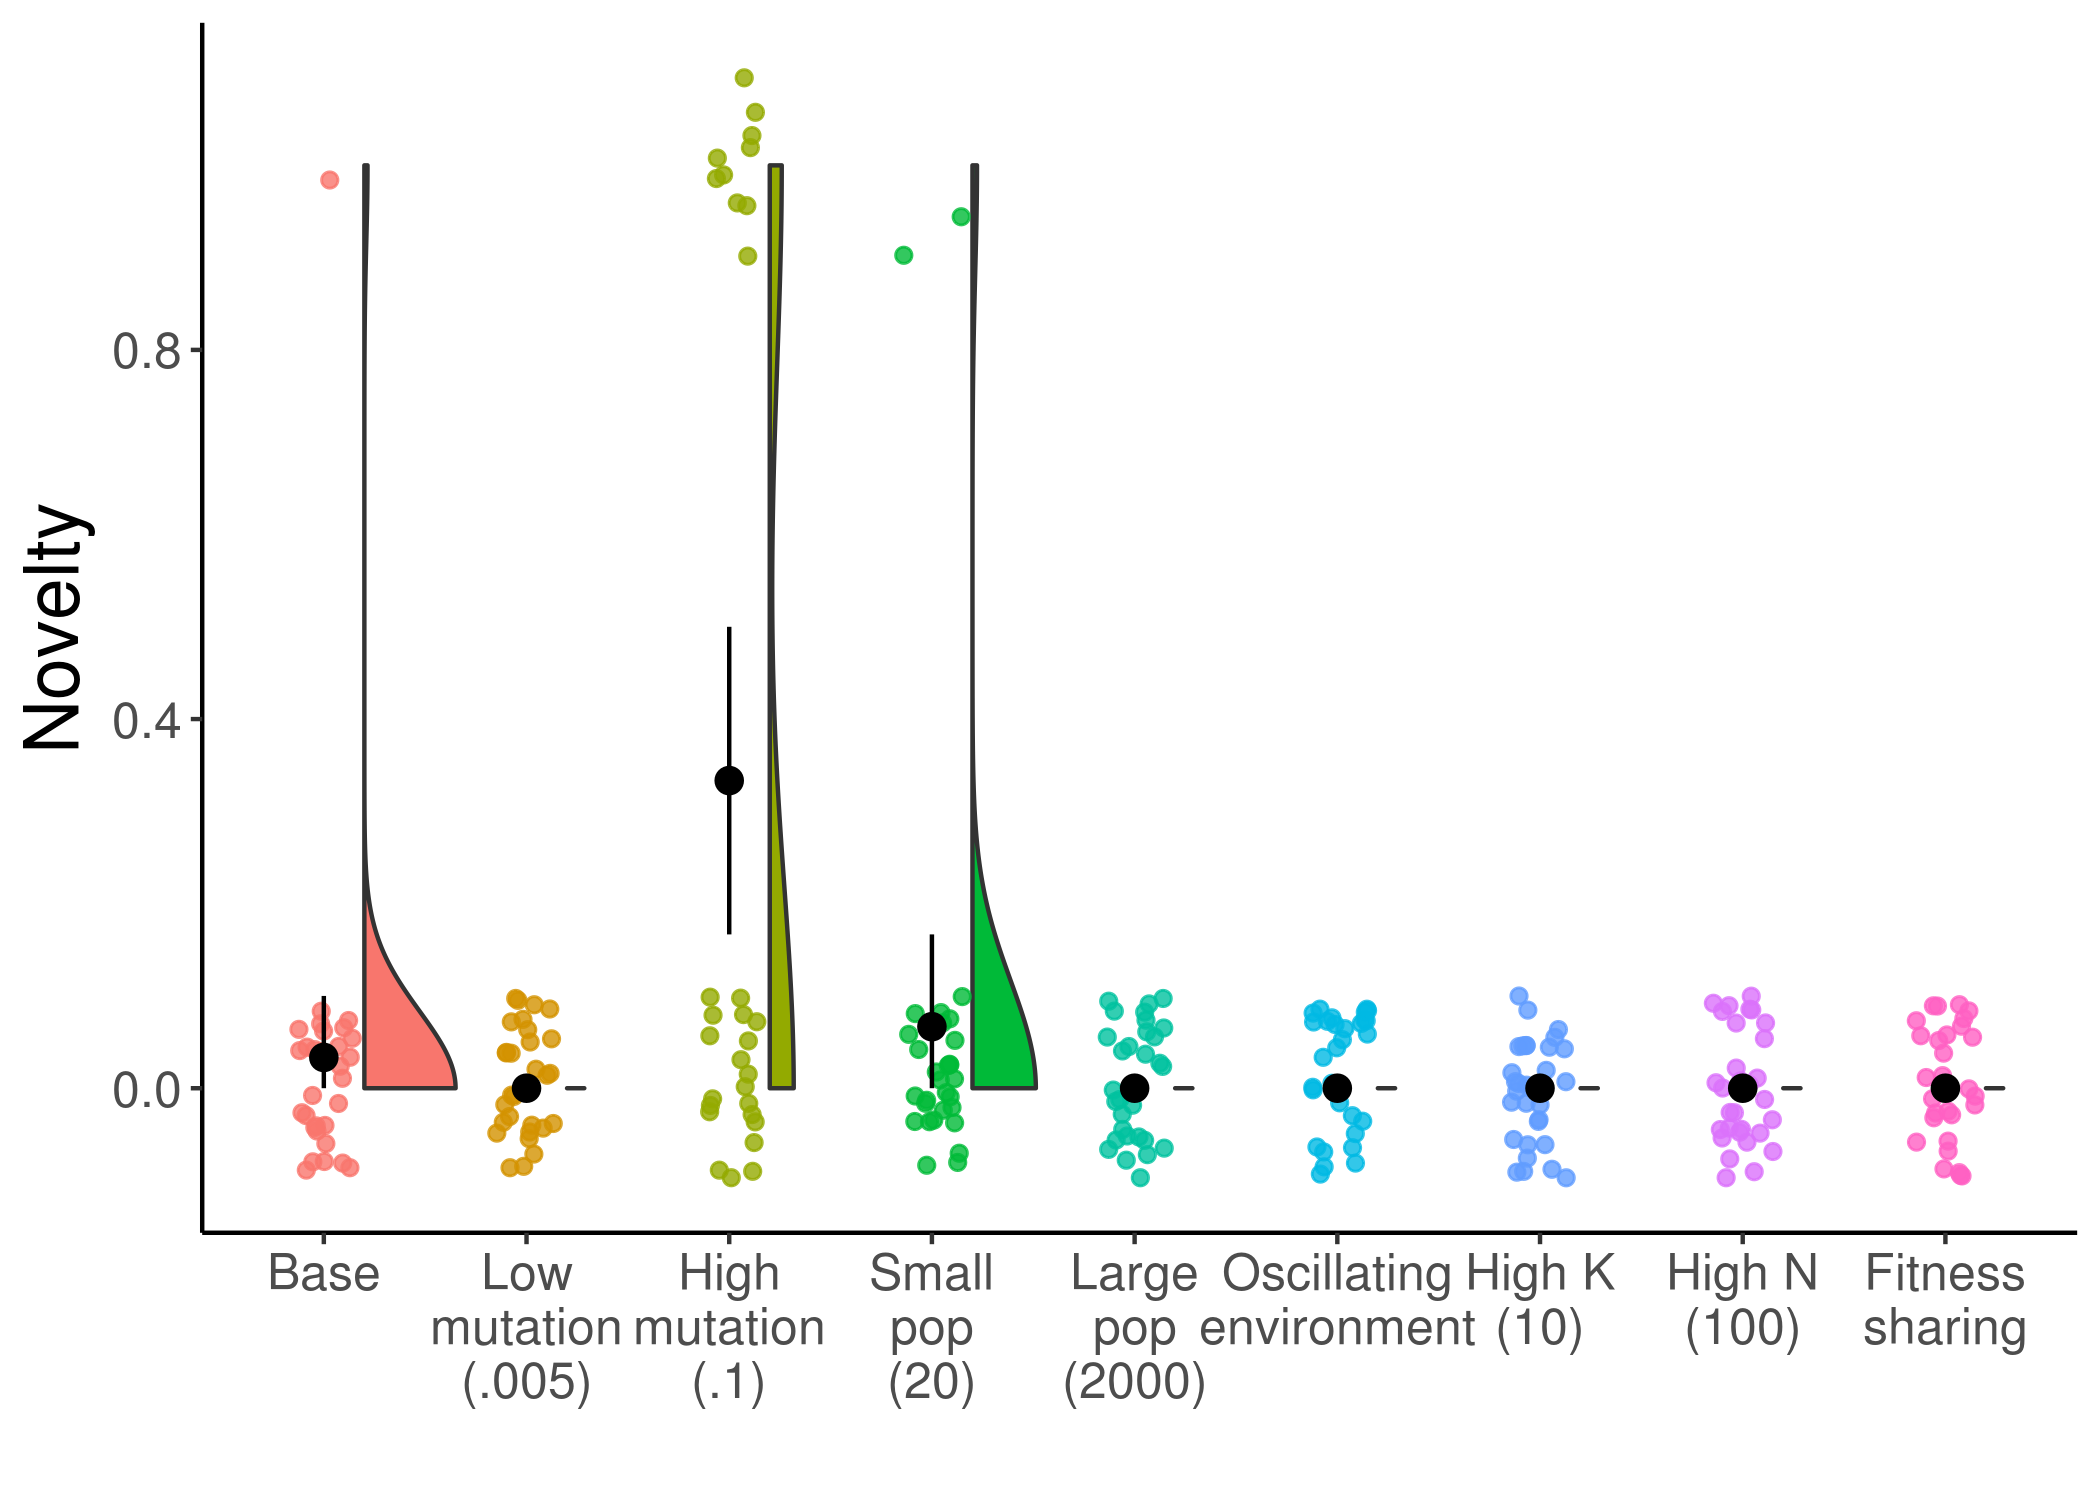
\includegraphics[width=3.5in]{figs/noveltyboxplots.png}
\caption{\textbf{Amount of novelty at final time point in varying environments.} At the final time point, no meaningful novelty is found in our baseline populations. However, increasing the amount of epistasis (K), increasing genome length (N), increasing mutation rate, decreasing population size, and enabling fitness sharing increase the amount of novelty produced in the final time point.}
\label{novelty}
\end{figure}

These results highlight the power of the novelty metric to identify environments and populations that have the potential to be open-ended due to the high number of new genotypes being consistently discovered. Novelty is likely necessary, but not sufficient, for open-ended evolution because if nothing new is being produced by a population, neither the complexity nor the ecological metric can be non-zero.

\subsection{Complexity Metric}
%The presence of highly complex organisms is a property of biological evolution that is often cited as something that artificial life systems have yet to achieve.  
Figure~\ref{complexity_time} shows the trajectories of the complexity metric over time in NK Landscape populations with and without fitness sharing. In our baseline NK treatment, organisms cannot evolve to be more complex than N. As a result, the complexity increases over time and then saturates. Conversely, fitness sharing leads to lower complexity because it weakens the pressure to be at the very top of a fitness peak (where complexity would be maximized).

\begin{figure}
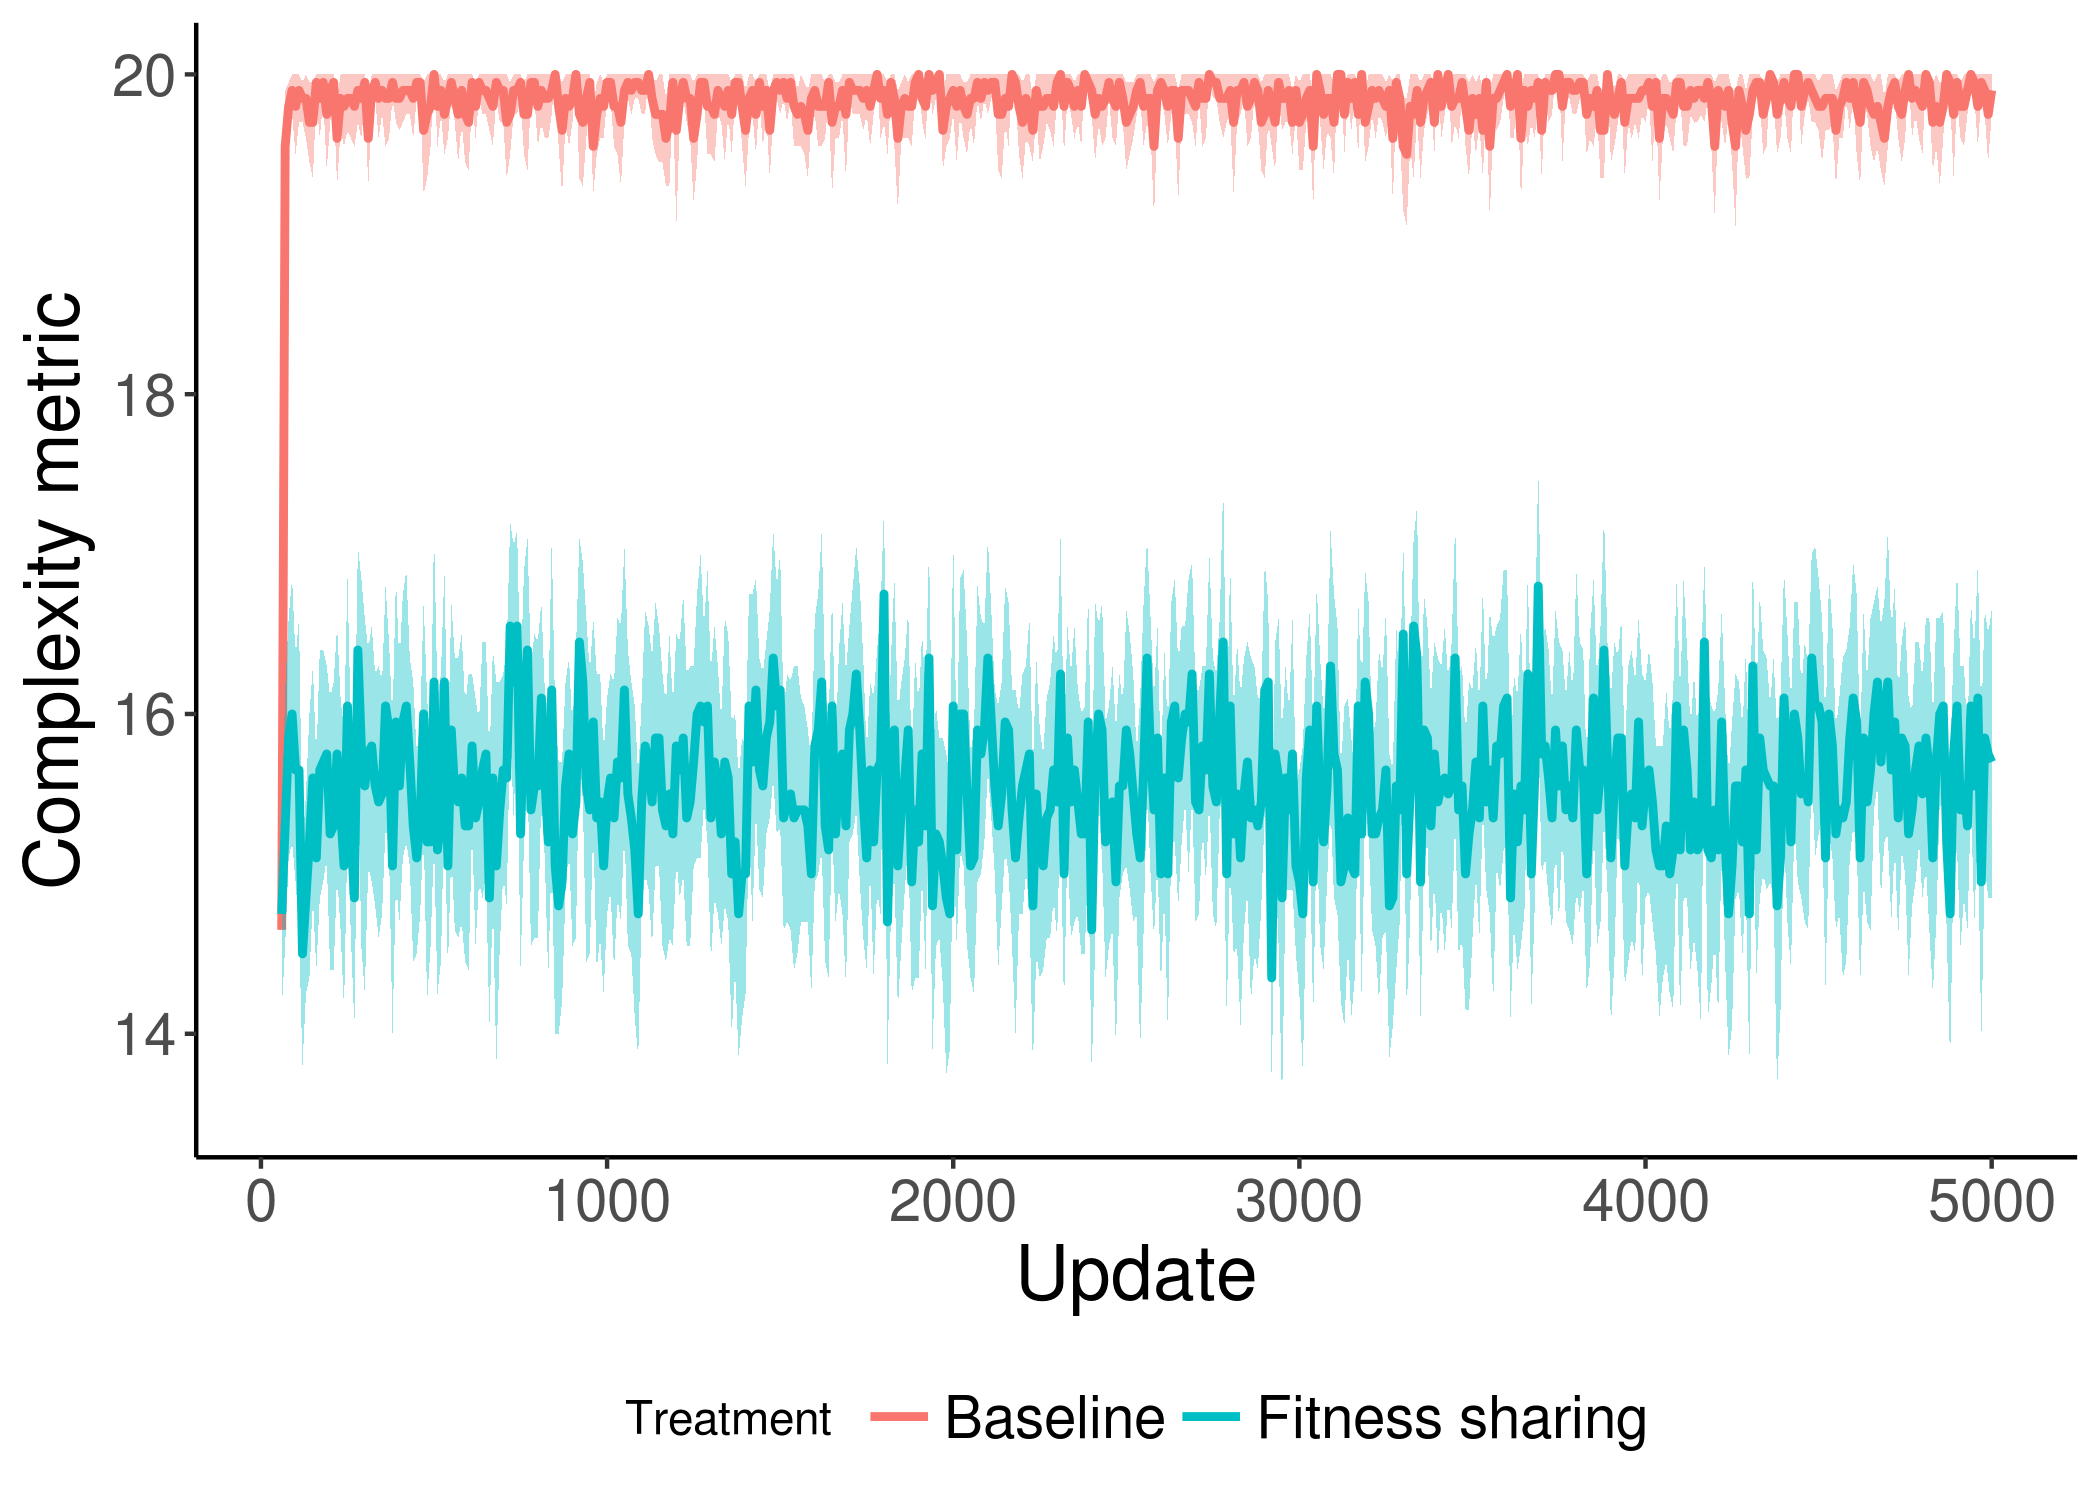
\includegraphics[width=3.5in]{figs/complexity_fitness_sharing.png}
\caption{\textbf{Amount of complexity over time in the baseline and fitness sharing NK Landscape conditions.} The baseline treatment (red) is able to reach the top complexity allowed by the model quickly and remain at that value. When fitness sharing is introduced (blue), the population is not able to attain the top complexity value. Shaded region represents a bootstrapped 95\% confidence interval around the mean.}
\label{complexity_time}
\end{figure}

Because of the simplicity of NK Landscapes, the complexity metric stabilizes quickly in most of those treatments and therefore we show only the final time point values for complexity in Figure~\ref{complexity}. The baseline treatment was able to reach the maximum complexity possible for a 20-bit genome and most of the environments did not decrease in the final complexity value. When the genome length was increased to 100 bits, the populations were also able to reach the new maximum complexity value of 100. However, high mutation rate, smaller population size, and fitness sharing all somewhat decreased the final complexity achieved on average. A high mutation rate decreased the final complexity because it introduced more deleterious mutations and therefore increased the percentage of the population that has just mutated away from the fitness peak at any point in time. A smaller population size decreased the complexity somewhat because smaller populations are more susceptible to genetic drift. As discussed previously, fitness sharing decreased the overall complexity achieved by the population due to the weakened selection for climbing fitness peaks when there are many organisms on that peak.

\begin{figure}
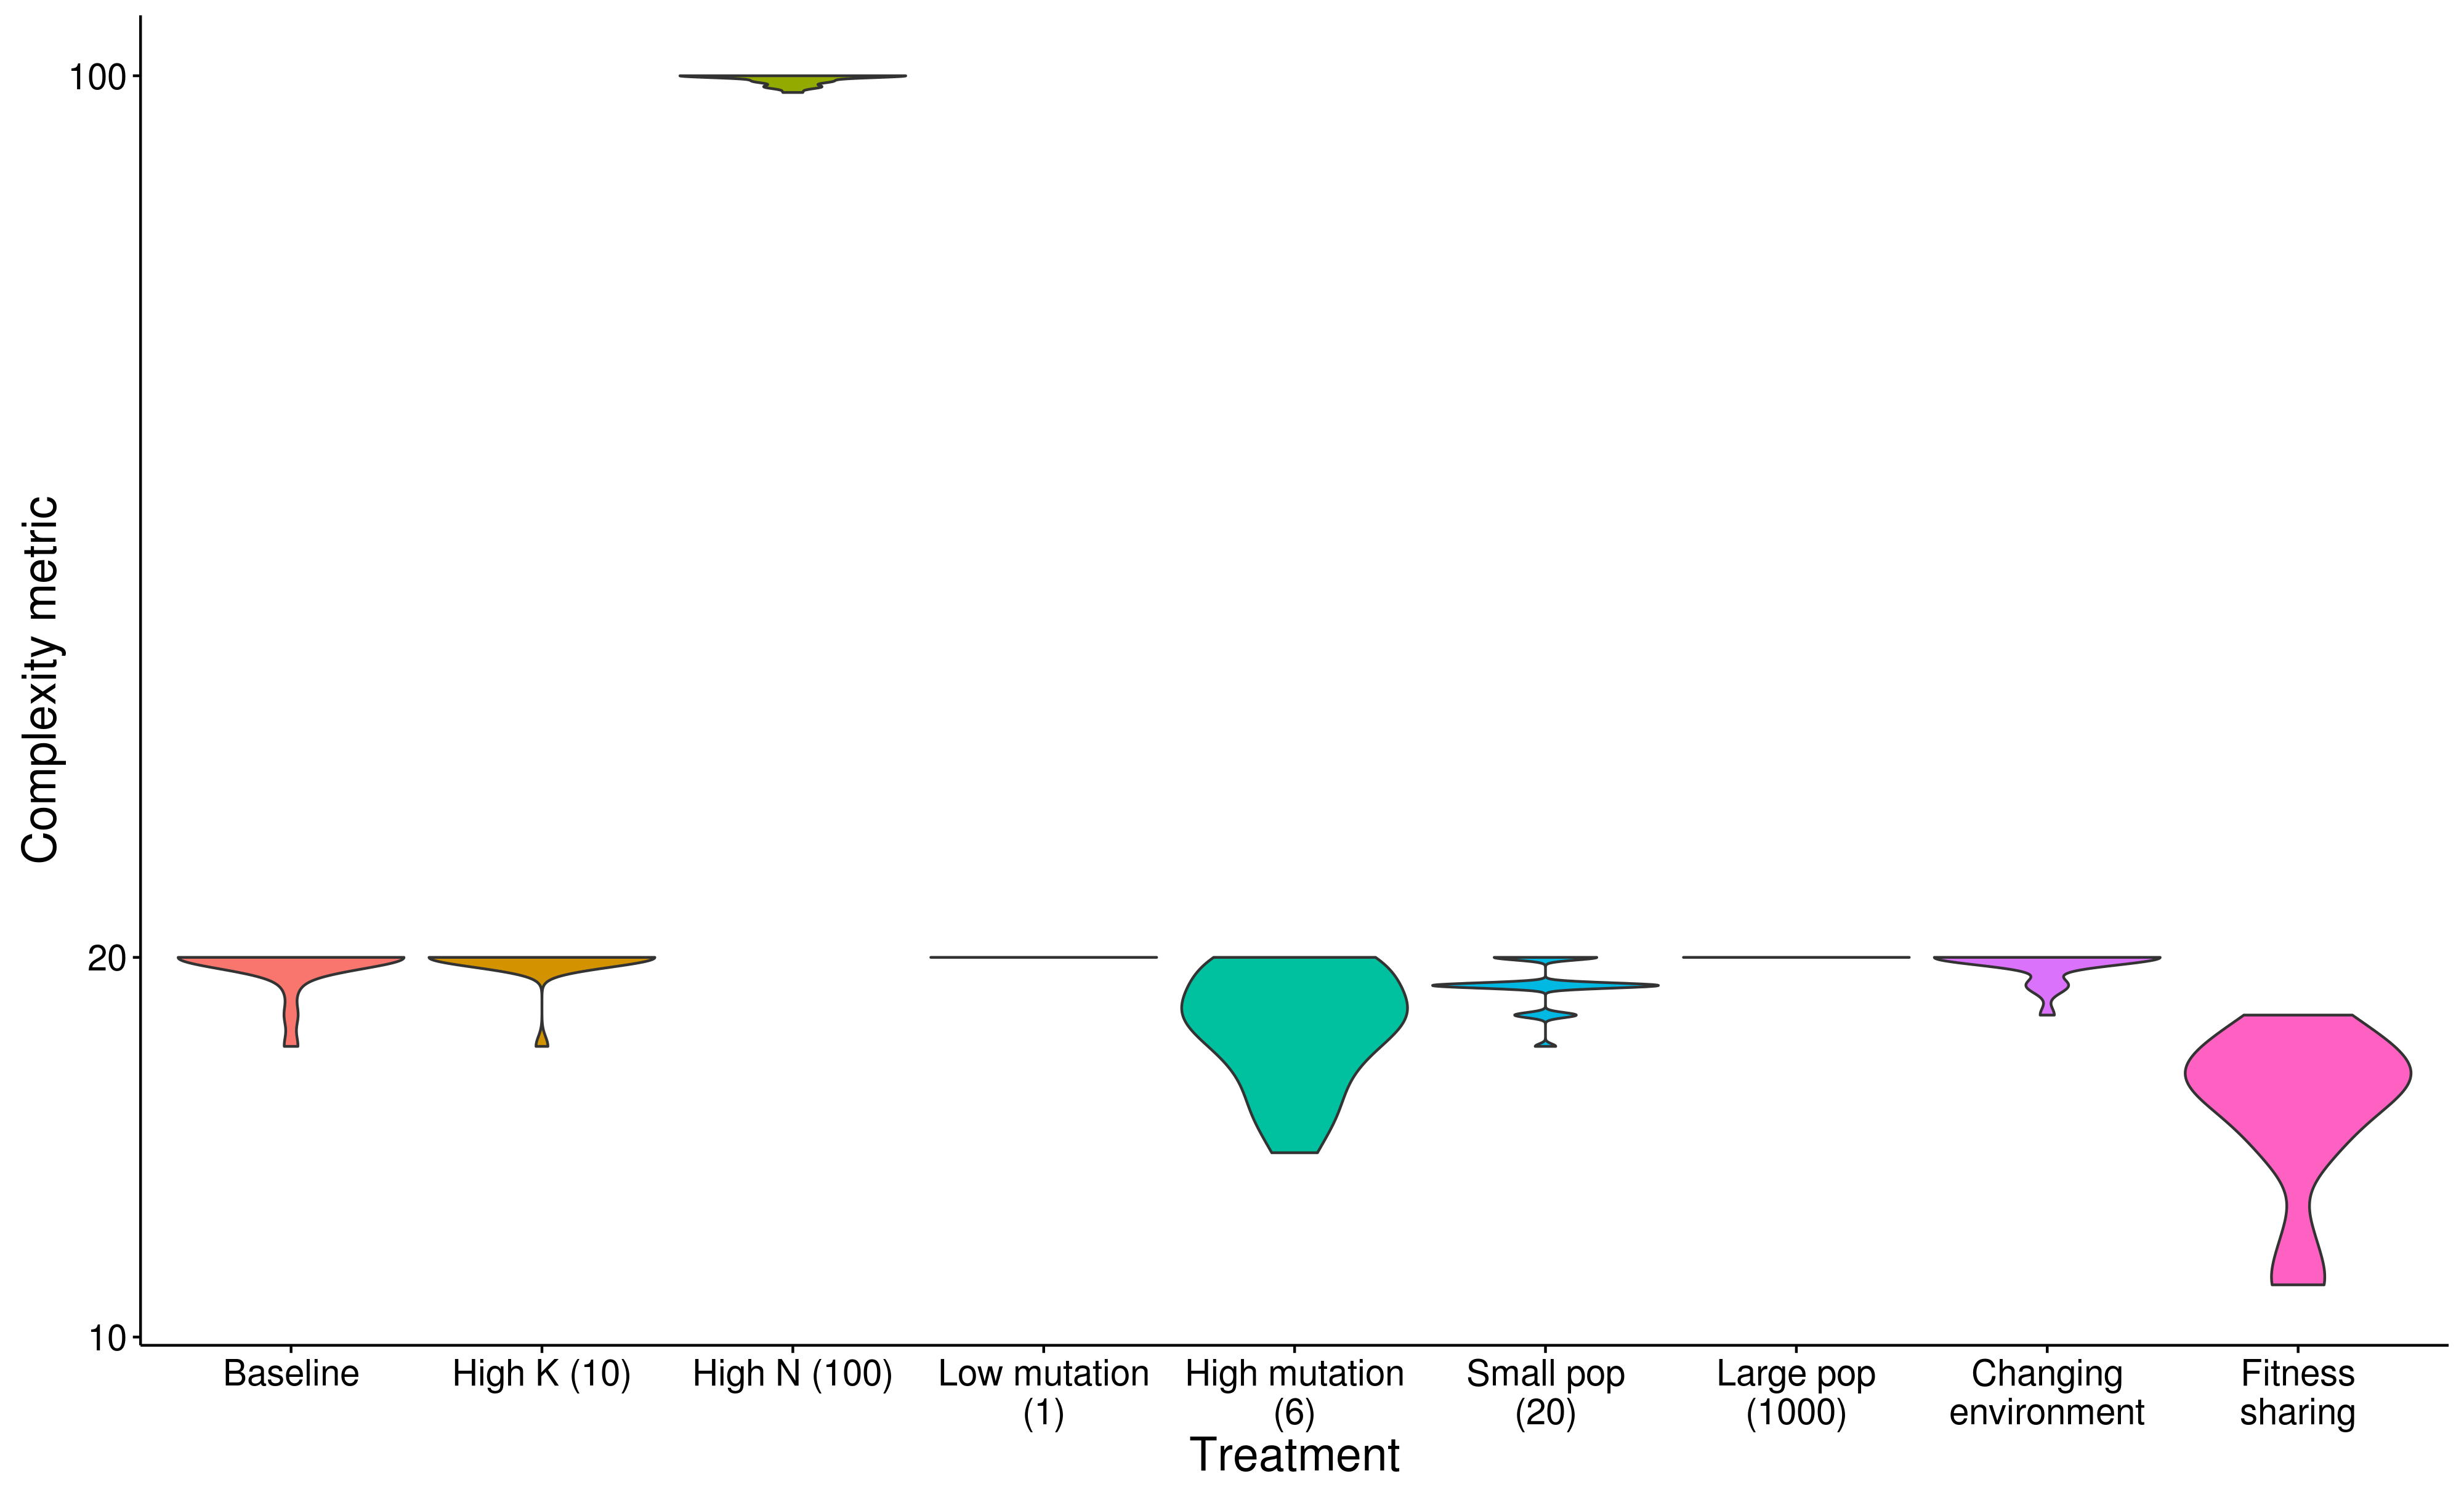
\includegraphics[width=3.5in]{figs/complexityboxplots.png}
\caption{\textbf{Amount of complexity at final time point in NK Landscape environments.} Most of the treatments reach the maximum complexity allowed by the genome length (20 or 100) and cannot continue to increase. High mutation rate, smaller populations, and fitness sharing decrease the final complexity achieved by the populations on average.}
\label{complexity}
\end{figure}

The NK Landscape results demonstrate that the complexity metric correctly identifies a system that is not able to continuously produce more complex solutions. Once the maximum complexity allowed by the genome length is reached, no higher value is possible. 

\begin{figure}
    \centering
    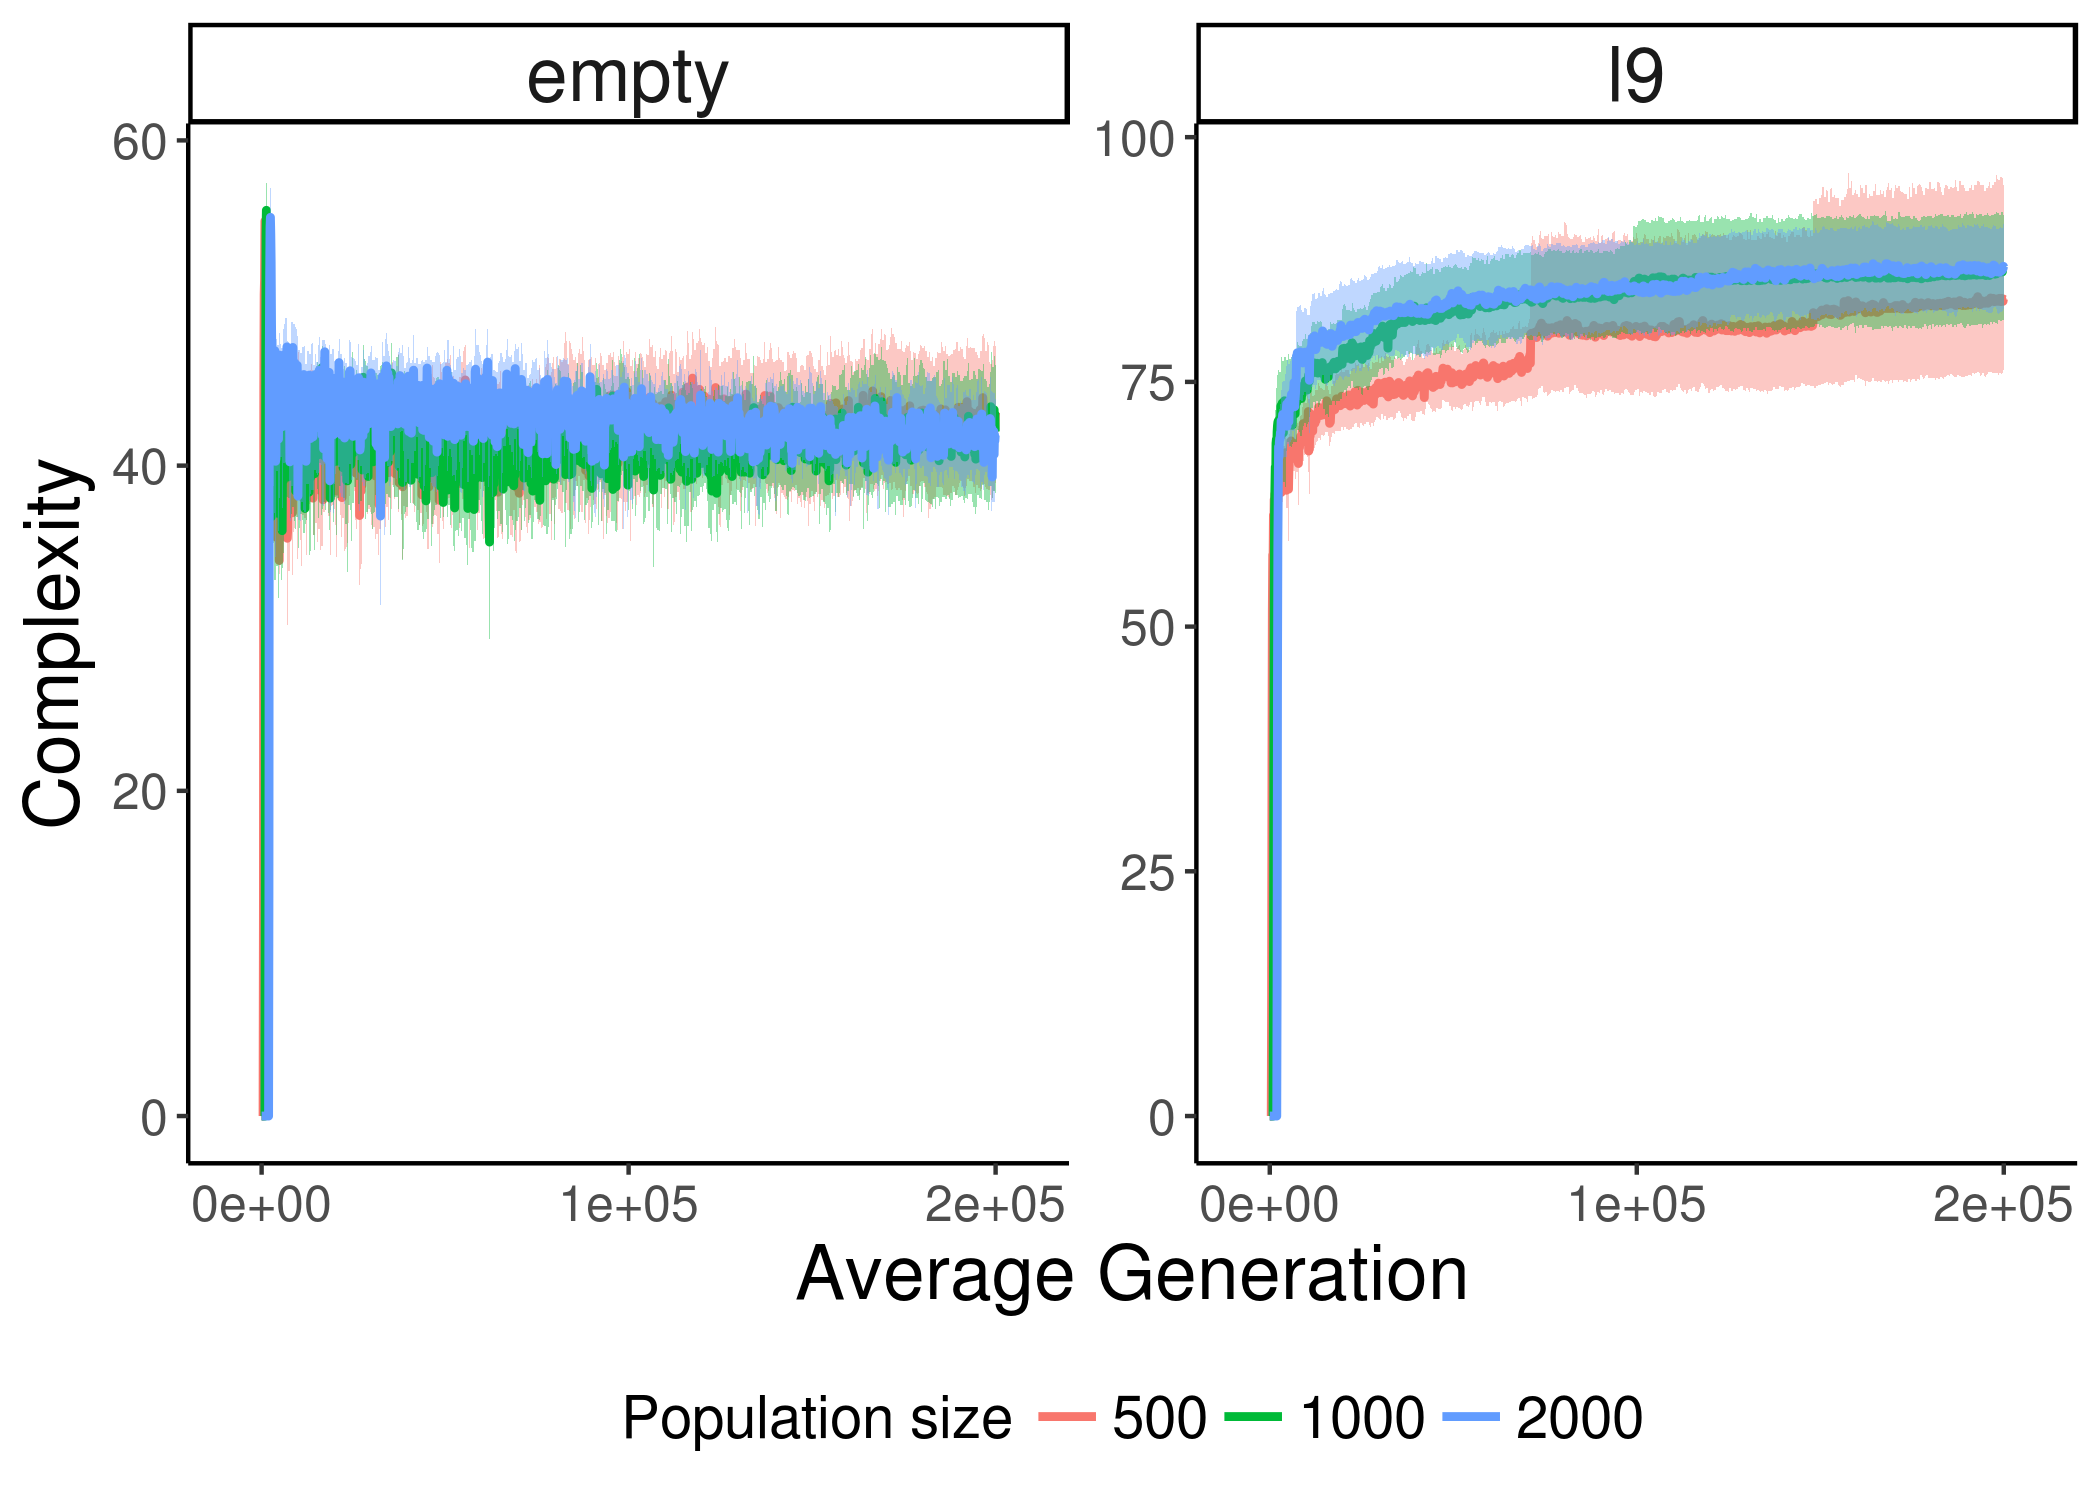
\includegraphics[width=3.5in]{figs/avida_env_complexity.png}
    \caption{\textbf{Complexity in Avida over time across different environments and population sizes.} Note that y axes have different scales.}
    \label{fig:avida_env_complexity}
\end{figure}

In Avida, the complexity metric reveals a stark difference between the empty and logic-9 environments. In the empty environment, there is a rapid rise in complexity followed by a decrease and leveling out. This behavior is likely due to the strong pressure in Avida to become a more efficient self-replicator by optimizing code. Over time, simpler solutions are selected for, all else being equal. In the logic-9 environment, on the other hand, there is an ongoing upward trajectory in complexity. While logic-9 still rewards efficiency, algorithms that can make maximally efficient use of the tasks are complex. These results are consistent with other measurements of complexity in Avida over time \citep{adami_evolution_2000}.

In the biosphere, complexity appears to be growing without bound \citep{Korb:2011kg}, although there is debate over the mechanisms behind this process. As such, building a non-trivial system that exhibits such behavior is a worthwhile goal for open-ended evolution research. Unbounded growth in complexity is only possible in a system with a sufficiently complex environment such that there is always new information to be integrated into the genome.

\subsection{Ecology Metric}
%Finally, a diverse population of interacting organisms promotes feedback loops that allow for the continuous creation of new and complex adaptations. Even if a system is not evolving more complex individual organisms, it may still be exhibiting interesting dynamics because it allows for a large number of niches that can be occupied by a diversity of organisms. Our ecology metric captures this dimension of open-ended evolution. 

Across both of our systems, the only condition that creates a multi-niche environment is the fitness sharing condition in NK Landscapes. Accordingly, that is the only condition in which we observe ecology greater than 1 Figure~\ref{ecology}. Because fitness sharing specifically rewards organisms with less common genotypes, it promotes a stably high ecology value over time. This result demonstrates the trade-off inherent in fitness sharing because it leads to higher ecology at the expense of lower complexity.

\begin{figure}
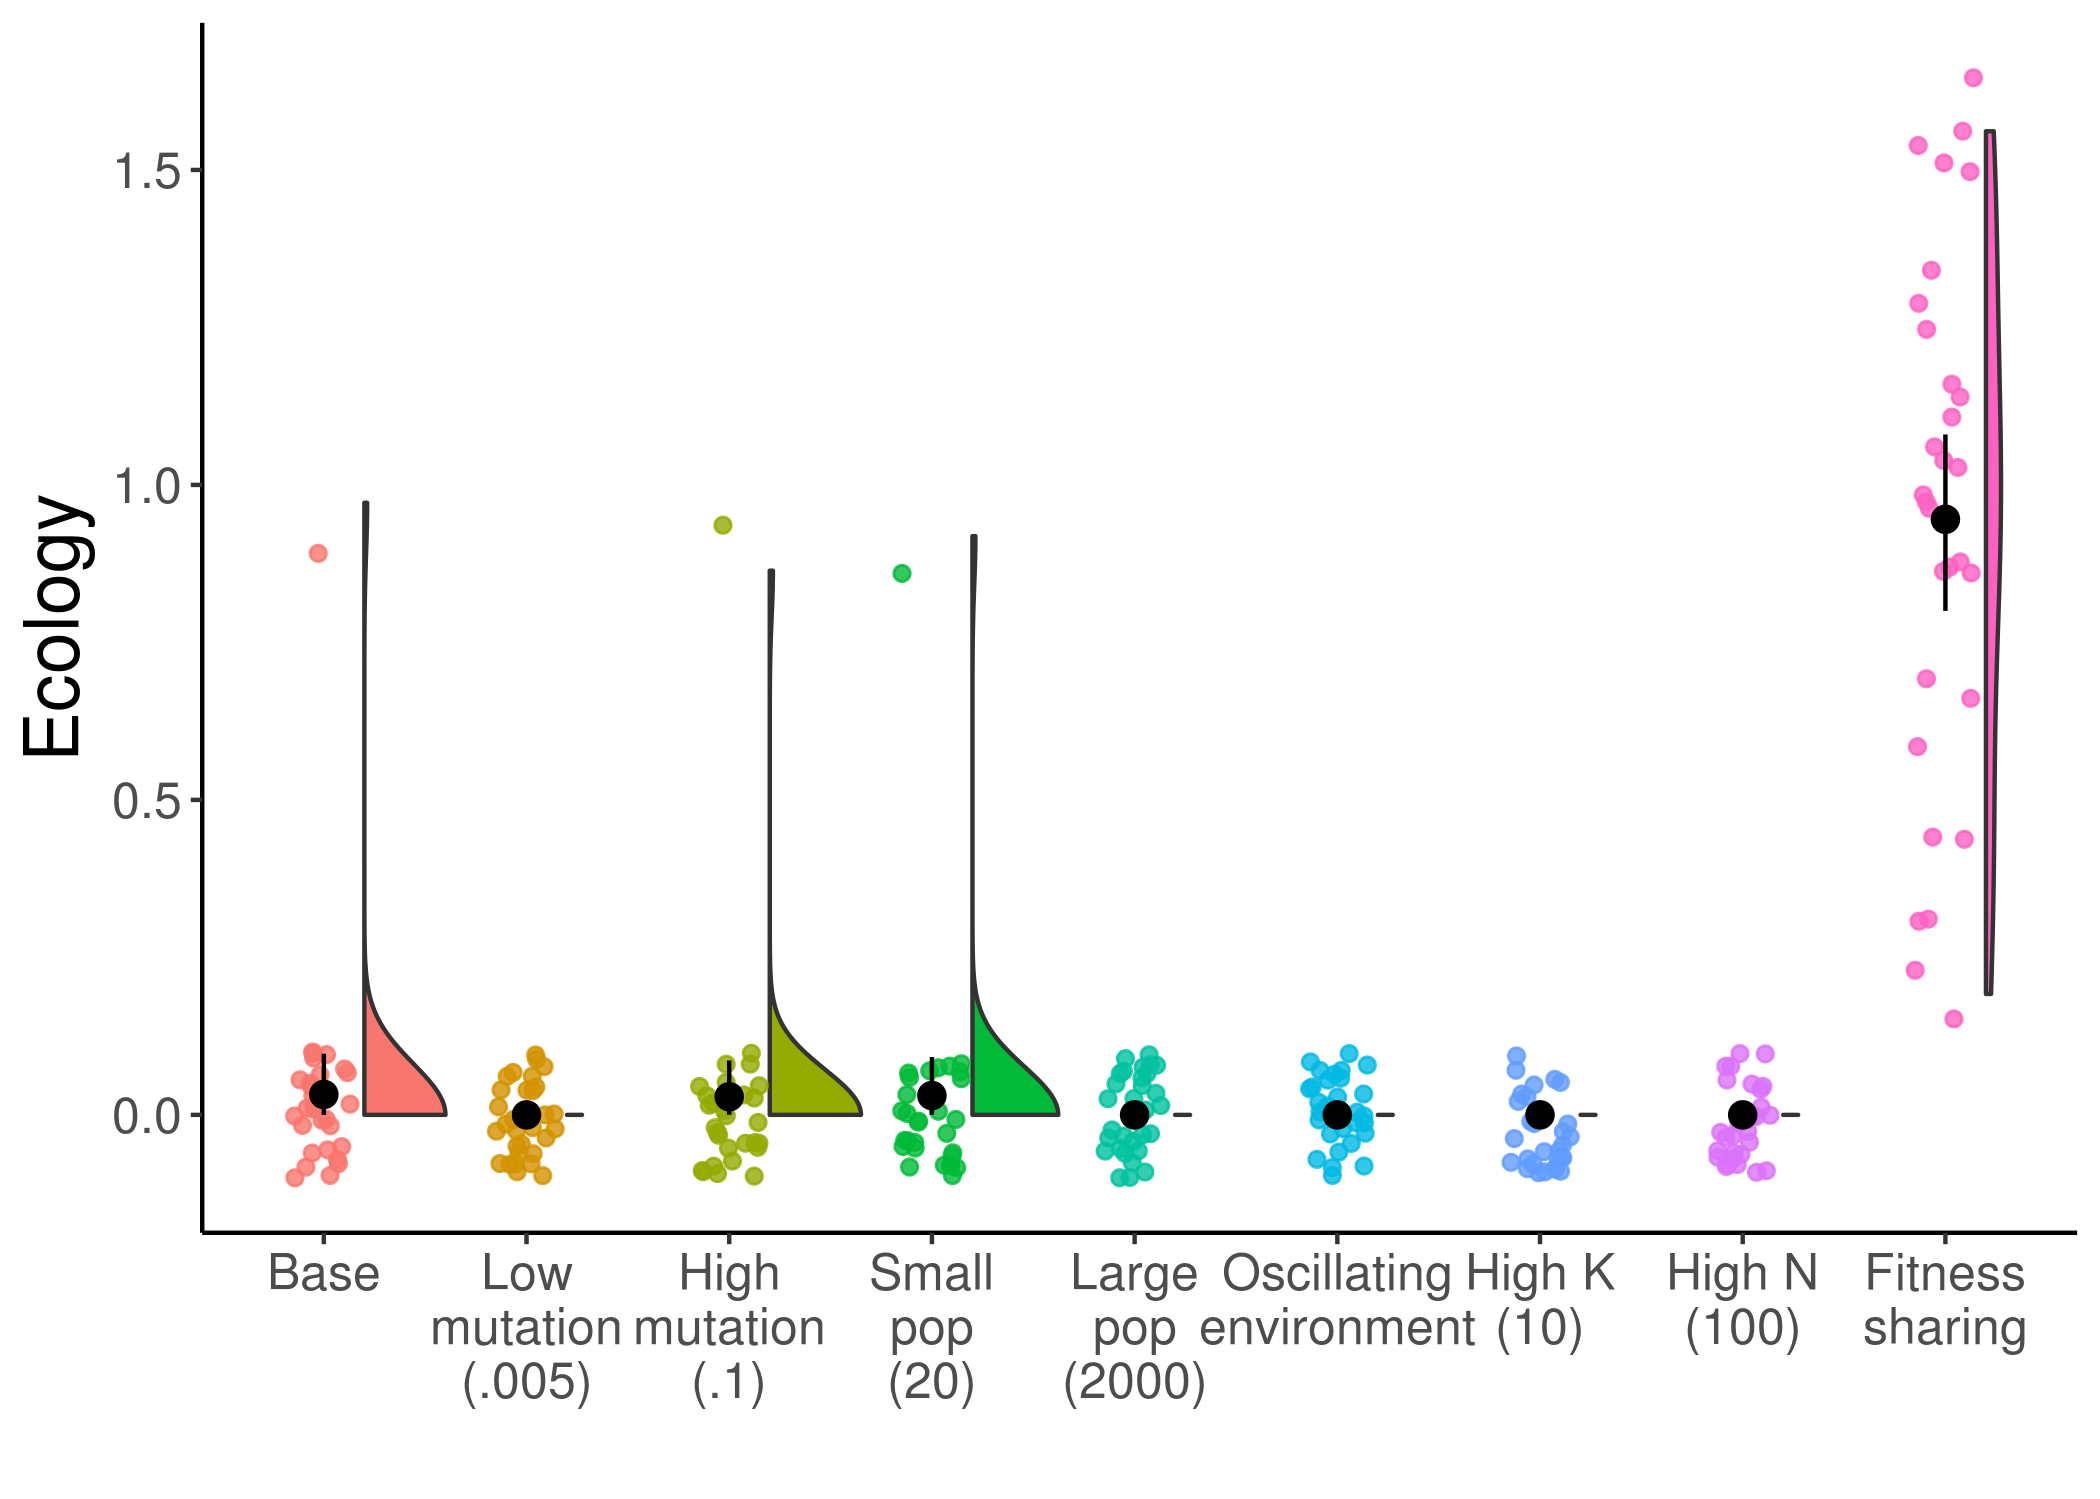
\includegraphics[width=3.5in]{figs/ecologyboxplots.png}
\caption{\textbf{Amount of ecology at final time point in varying environments.} }
\label{ecology}
\end{figure}

%Interestingly, increasing the complexity of the environment by adding tasks has a relatively small impact on change, likely due to the fact that, despite its increased complexity, \textbf{logic-9} is still a single niche environment. According to coalescence theory, if we used a large enough value of $t$, 

%We hypothesize that a continuously increasing ecology metric in addition to a continuously increasing complexity metric are necessary for an evolutionary system to truly be open-ended as we observe in the biosphere.

Ecology is an incredibly powerful force in nature, leading to feedback cycles of ever-increasing diversity. Like complexity, diversity seems to be growing without bound in the biosphere \citep{harmon_species_2015}. Thus, it will be important to see what mechaisms are important to promoting it in artificial life systems, too.

\section{Conclusions}
We have proposed a suite of metrics that quantify the presence of four generally-accepted hallmarks of evolution. These metrics build on prior work on evolutionary activity statistics and are largely compatible with them. Additionally, we have proposed techniques for reducing noise in these statistics.  By testing them on two very different well-understood evolutionary systems, we have demonstrated that our metrics respond in an intuitive way to the dynamics these systems exhibit. Thus, these metrics should also be useful in understanding the extent to which novel systems exhibit hallmarks of open-ended evolution. Moreover, we can use them to understand the impact of incremental changes to a system. By breaking the seemingly monolithic problem of designing an open-ended evolutionary system into smaller, measurable pieces, we facilitate improved use of the scientific method. One of the primary goals in building an open-ended evolutionary system is to understand what components are necessary to do so. By looking at the effects that individual, controlled changes to a system have on this suite of metrics, we can more effectively work towards these goals.

Going forward, it will be interesting to see how a wider variety of artificial life systems respond to the metrics in the MODES toolbox. In particular, further investigation on the differences between using a shadow run as a filter and using the persistence filter described here would be highly worthwhile. Ultimately, these two techniques capture sufficiently different information that it may be valuable to use each in turn.

%First, it is clear that for new behaviors to evolve in a system, new genomes need to be evolving. Therefore, both the change and novelty metrics would need to be non-zero -- though they could be stable instead of increasing since both metrics measure a change. 

%Second, continuously increasing maximum complexity with a stable environment would imply increasing biotic interactions, potentially cooperative or complex competitive interactions. If maximum complexity is increasing in a population, at least one organism must be incorporating more information into its genome than any organism had before. This information can be about the environment up to a point. However, if the environment is not changing, maximum complexity will not be able to increase unboundedly without biotic interactions between organisms. Therefore, continuously increasing maximum complexity implies that interesting biotic interactions are evolving in a system.

%Finally, a continuously increasing ecological metric in a stable environment implies an ecosystem is forming; if the ecology metric is increasing, the informative diversity in the population is increasing. For diversity to be increasing, new niches must be emerging -- if there were only a single niche, the best genotype for that niche would fill it and take over the population. The only way for diversity to be maintained for a meaningful length of time is for new niches to be created. While new niches can emerge from abiotic factors, if the environment is not changing, those will all eventually fill. Therefore, the only way for an indefinite series of new niches to form (which is required for an unbounded increase of the ecological metric), is via biotic interactions between organisms in the population. Those biotic interactions could fall into a number of categories such as predator and prey, mutualism, parasitism, or commensalism, but as the number of them increase, a complex ecosystem emerges.

For a long time, the field of open-ended evolution has been plagued by a lack of data that is comparable between systems. We believe that the MODES toolbox will help remedy this problem by making generally applicable metrics easily accessible. As new hallmarks of open-ended evolution are identified and new techniques of filtering noise out of populations are developed, we encourage contributions to the toolbox. By working together as a community of users, researchers, and developers we can dramatically increase the rate at which open-ended evolution research progresses.

%TODO: We need something more here

\section{Acknowledgments}
We thank members of the MSU Digital Evolution Lab for helpful feedback on this manuscript. This research was supported by the National Science Foundation (NSF) through the BEACON Center (Cooperative Agreement DBI-0939454), a Graduate Research Fellowship to ED (Grant No. DGE-1424871), and NSF Grant No. DEB-1655715 to CO. Michigan State University provided computational resources through the Institute for Cyber-Enabled Research and the Digital Scholarship Lab. Any opinions, findings, and conclusions or recommendations expressed in this material are those of the author(s) and do not necessarily reflect the views of the NSF or MSU.

\bibliographystyle{apalike}
\bibliography{zotero,bibliography}

\end{document}
